% указываем класс документа
\documentclass[12pt,a4paper,openany]{extarticle}

% подключаем собственный стилевой файл 
\usepackage{mystyle}

% указываем язык (для автоматической вставки слов, типа "Глава", "Содержание", "Литература", "рис." и пр.
\selectlanguage{russian}


\begin{document}

\newcounter{myappcounter}
\renewcommand{\themyappcounter}{\Alph{myappcounter}}
\newcommand{\myappnum}{\refstepcounter{myappcounter}\themyappcounter}

\part*{Лабораторная работа №5\\
Разработка системы управления для неполноприводного робота.\\ {\LARGE Часть~2.~Расчет коэффициентов регулятора.}}

\section{Теоретические сведения}

\paragraph*{Введение}$\phantom{-}$\\
\hspace*{\parindent}В~первой части пособия по данной работе для обоих роботов было получено следующее уравнение, описывающее их работу:
\begin{equation}\label{dx=Ax+Bu}
	\dot x = Ax + Bu\ldotp
\end{equation}
Дополнив его еще одним соотношением можно получить систему матричных уравнений, называемую \textit{моделью <<вход-состояние-выход>>} исследуемого объекта управления:
\begin{equation}
	\left\{
	\begin{aligned}
		\!&\dot x = Ax + Bu \\
		\!&y = Cx,
	\end{aligned}
	\right.
\end{equation}
где 
$x$~--- $n$-мерный вектор состояния системы ($n$~--- количество переменных в векторе состояния (в нашем случае $n=3$); также $n$ называют \textit{порядком объекта управления}); \\
$y$~--- $l$-мерный вектор выходных величин ($l$~--- количество переменных в нем);\\
$u$~--- $m$-мерный вектор управляющих воздействий ($m$~--- количество переменных в нем (в нашем случае $m=1$));\\
$A$~--- матрица, определяющая динамические свойства объекта управления, размерности $n\times n$;\\
$B$~--- матрица входа управляющих воздействий размерности $n\times m$;\\
$C$~--- матрица выхода размерности $l\times n$, определяющая, какие из компонент вектора состояния, или какие их линейные комбинации будут рассматриваться как выходные величины (сигналы) объекта управления (например, если в качестве $y$ следует взять только величины $\psi$ и $\dot\psi$, то матрица $C$ будет равна:
\begin{equation}
	C = 
	\begin{bmatrix}
		1 & 0 & 0\\
		0 & 0 & 1
	\end{bmatrix}\!\!;
\end{equation}
проверяя:
\begin{equation}
y = Cx = 
\begin{bmatrix}
		1 & 0 & 0\\
		0 & 0 & 1
\end{bmatrix}
\begin{bmatrix}
\psi \\ \dot\theta \\ \dot\psi
\end{bmatrix}
=
\begin{bmatrix}
\psi  \\ \dot\psi
\end{bmatrix}\!\!,
\end{equation}
убеждаемся, что в этом случае $y$ действительно будет равен $[\psi\;\dot\psi]^T$).

Прежде, чем приступить к каким-либо расчетам, необходимо проверить, а возможно ли вообще управлять исследуемым объектом.
Для этих целей в рассмотрение вводится так называемая \textit{матрица управляемости} $Y$\!, формируемая как\footnote{Данная запись означает, что упоминаемые матрицы следует записать рядом и полученный результат рассматривать как новую матрицу.
Например,
\begin{equation*}
	O_1=
	\begin{bmatrix}
		1 & 2\\
		3 & 4
	\end{bmatrix}\!\!,\quad
	O_2=
	\begin{bmatrix}
		9\\
		8 
	\end{bmatrix}\!\!,\quad
	O_3 = [O_1\ O_2] =
	\begin{bmatrix}
		1 & 2 & 9\\
		3 & 4 & 8
	\end{bmatrix}\!\!\ldotp
\end{equation*}}
\begin{equation}
	Y = 
	\begin{bmatrix}
		B & AB & A^2B & \dots & A^{n-1}B
	\end{bmatrix}\!\!,	 
\end{equation}
и вычисляется ее определитель. 
В~случае, если $\det Y\ne0$, система управляема и синтез регулятора возможен. 
Иначе остается заключить, что рассматриваемый объект неуправляем.

\paragraph*{Расчет коэффициентов регулятора}$\phantom{-}$\\
\hspace*{\parindent}Для управления роботами, описанными в первой части данного пособия, предлагается использовать \textit{пропорциональный регулятор состояния (П-регулятор состояния)}, формирующий управляющее воздействие\footnote{Для рассматриваемых роботов управляющим воздействием является напряжение $U$, подаваемое на их двигатели.} согласно формуле:
\begin{equation}\label{eq:control_law_main}
u = Ke,
\end{equation}
где $K$~--- матрица коэффициентов регулятора, равная
\begin{equation}
K = 
\begin{bmatrix}
	k_1 & k_2 & k_3
\end{bmatrix}\!\!,
\end{equation}
а $e$~--- вектор ошибок, определяемый как
\begin{equation}
e = x_w-x = 
\begin{bmatrix}
\psi_w \\ \dot\theta_w \\ \dot\psi_w
\end{bmatrix}
-
\begin{bmatrix}
\psi \\ \dot\theta \\ \dot\psi
\end{bmatrix}\!\!,
\end{equation}
где в свою очередь $x_w$~--- вектор, содержащий желаемые значения компонентов вектора состояния.
Поскольку желаемое поведение изучаемых роботов описывается нулевым вектором~$x_w$:
\begin{equation}
x_w = 
\begin{bmatrix}
0 & 0 & 0
\end{bmatrix}^T\!\!\!\!,
\end{equation} 
то выражение~\eqref{eq:control_law_main} будет эквивалентно следующему:
\begin{equation}\label{eq:control_law_simple}
u = -Kx\ldotp
\end{equation}

Подставив~\eqref{eq:control_law_simple} в~\eqref{dx=Ax+Bu} можно получить:
\begin{equation}\label{eq:dx_Fx}
\dot x = Ax - BKx = (A - BK)x = Fx,
\end{equation}
где $F=A-BK$.
Введя для компонент матриц $A$ и $B$ следующие обозначения
\begin{equation}\label{eq:compose_of_A_B}
A = 
\begin{bmatrix}
0      & 0      & 1\\
a_{21} & a_{22} & 0\\
a_{31} & a_{32} & 0
\end{bmatrix}\!\!,\qquad\qquad
B = 
\begin{bmatrix}
0 \\ b_2 \\ b_3
\end{bmatrix}\!\!,
\end{equation}
состав матрицы $F$ можно представить так: 
\begin{equation}\label{eq:F_through_A_B}
F = 
\begin{bmatrix}
0      & 0      & 1\\
a_{21} & a_{22} & 0\\
a_{31} & a_{32} & 0
\end{bmatrix}
-
\begin{bmatrix}
0 \\ b_2 \\ b_3
\end{bmatrix}
\begin{bmatrix}
	k_1 & k_2 & k_3
\end{bmatrix}
=
\begin{bmatrix}
0             & 0             & 1\\
a_{21}-b_2k_1 & a_{22}-b_2k_2 & -b_2k_3\\
a_{31}-b_3k_1 & a_{32}-b_3k_2 & -b_3k_3
\end{bmatrix}\!\!\ldotp
\end{equation}
Для сокращения дальнейших записей введем обозначение, аналогичное~\eqref{eq:compose_of_A_B}:
\begin{equation}\label{eq:compose_of_F}
F = 
\begin{bmatrix}
0      & 0      & 1\\
f_{21} & f_{22} & f_{23}\\
f_{31} & f_{32} & f_{33}
\end{bmatrix}\!\!\ldotp
\end{equation}

Поведение исследуемой системы зависит от вида \textit{характеристического полинома} матрицы~$F$\footnote{Это можно проиллюстрировать хотя бы тем фактом, что с точностью до замены $\lambda^v$ на $\dfrac{d^v\psi}{dt^v}$ или $\dfrac{d^v\omega}{dt^v}$ характеристический полином матрицы~$F$ совпадает с левой частью дифференциальных уравнений относительно функций $\psi(t)$ и $\omega(t)$, получающихся из системы~\eqref{eq:dx_Fx} (см.~Приложение~\ref{append:some_maths}).}:
\begin{equation}
	D(\lambda) = \det(\lambda E - F) = \lambda^3 + z_{2}\lambda^{2} + z_{1}\lambda + z_0,
\end{equation}
где $\lambda$~--- <<обычная>> (никак не определяемая) переменная; $E$~--- единичная матрица; $z_i$~($i\in\{0,1,2\}$)~--- числовые коэффициенты, получающиеся при расчете.
При этом требуемому поведению системы~--- поддержке нулевых значений компонент вектора~$x$, определенному ее быстродействию и проч.~--- будет соответствовать определенный вид (определенные значения коэффициентов $z_i$) характеристического полинома:
\begin{equation}\label{poly_needed}
	D^*(\lambda) = \lambda^3 + z^*_2\lambda^2 + z_1^*\lambda + z^*_0\ldotp
\end{equation}

Последний полином задается разработчиком в соответствии с тем, какие характеристики (какое поведение) он хочет видеть у разрабатываемой системы.
При этом (опять же в зависимости от желаемого поведения системы) применяются различные методы расчета постоянных коэффициентов $z^*_i$ ($i\in\{0,1,2\}$).
В~данной работе их значения следует получить раскрытием по биному Ньютона выражения
\begin{equation}\label{poly's}
	D^*(\lambda) = (\lambda+w_0)^n\!\!,
\end{equation}
где $w_0$~--- числовое значение, рассчитываемое по формуле
\begin{equation}
	w_0 = \frac{t^*_\text{п}}{t_\text{п}},
\end{equation}
где, в свою очередь,  $t_\text{п}^*$~--- <<стандартное>> значение \textit{времени переходного процесса}, определяемое по порядку объекта управления  из таблицы~\ref{tabl};  $t_\text{п}$~--- <<действительное>> значение времени переходного процесса в нашей системе.
Для первого раза последнее можно взять равным, например, $0.5$~c.
В~данной работе под этими параметрами следует понимать некоторые величины, обратно пропорциональные быстродействию робота.
То есть, к примеру, уменьшение параметра $t_\text{п}$ при расчетах будет означать, что коэффициенты регулятора, получающиеся в результате, будут обеспечивать большее быстродействие технической системы.

\begin{table}[h!]
\caption{Значения параметра $t_\text{п}^*$ в зависимости от порядка объекта управления.}
	\label{tabl}
	\begin{equation*}
		\begin{array}{|c|c|c|c|c|c|c|}\hline
			\phantom{aa}n\phantom{aa} & \phantom{aa}1\phantom{aa} & \phantom{aa}2\phantom{aa} & \phantom{aa}3\phantom{aa} & \phantom{aa}4\phantom{aa} & \phantom{aa}5\phantom{aa} & \phantom{aa}6\phantom{aa} \\ \hline
			t_\text{п}^*,\text{ c} & 3.0 & 4.8 & 6.3 & 7.8 & 9.2 & 10.5 \\\hline
		\end{array}
	\end{equation*}
\end{table}

Характеристический полином матрицы $F$ будет равен заданному разработчиком, если будет справедливым соотношение
\begin{equation}\label{D(l)=D*(l)}
D(\lambda) = D^*(\lambda),
\end{equation}
в более подробном виде для нашего случая расписываемое как
\begin{gather}
\det(\lambda E - F) = (\lambda+w_0)^3,\\
%
\lambda^3 + z_{2}\lambda^{2} + z_{1}\lambda + z_0 = \lambda^3 + z^*_2\lambda^2 + z_1^*\lambda + z^*_0,\\
%
\lambda^3 - (f_{22}+f_{33})\lambda^2 + (f_{22}f_{33} - f_{23}f_{32} - f_{31})\lambda + (f_{22}f_{31} - f_{21}f_{32}) =
\lambda^3 + 3w_0\lambda^2 + 3w_0^2\lambda + w_0^3\ldotp
\end{gather}
Оно равносильно системе 3 алгебраических уравнений:
\begin{equation}
\left\{
\begin{aligned}
	\!&-f_{22}-f_{33} = 3w_0 \\
	\!&f_{22}f_{33} - f_{23}f_{32} - f_{31} = 3w_0^2\\
	\!&f_{22}f_{31} - f_{21}f_{32} = w_0^3,
\end{aligned}
\right.
\end{equation}
решением которой с учетом выражений~\eqref{eq:F_through_A_B} и~\eqref{eq:compose_of_F}:
\begin{align}
&\left\{
\begin{aligned}
	\!&-a_{22} + b_2k_2 +b_3k_3 = 3w_0 \\
	\!&(a_{22}-b_2k_2)(-b_3k_3)+b_2k_3(a_{32}-b_3k_2)-a_{31} + b_3k_1 = 3w_0^2\\
	\!&(a_{22}-b_2k_2)(a_{31}-b_3k_1)-(a_{21}-b_2k_1)(a_{32}-b_3k_2) = w_0^3,
\end{aligned}
\right.\\
%
&\left\{
\begin{aligned}
	\!&b_2k_2 + b_3k_3 = 3w_0 + a_{22}\\
	\!&b_3k_1 + (a_{32}b_2-a_{22}b_3)k_3 = 3w_0^2+a_{31}\\
	\!&(a_{32}b_2-a_{22}b_3)k_1 + (a_{21}b_3-a_{31}b_2)k_2 = w_0^3-a_{22}a_{31}+a_{21}a_{32}
\end{aligned}
\right.\\
%
\begin{bmatrix}
k_1 \\ k_2 \\ k_3
\end{bmatrix}
=
&\begin{bmatrix}
0                   & b_2                 & b_3\\
b_3                 & 0                   & a_{32}b_2-a_{22}b_3\\
a_{32}b_2-a_{22}b_3 & a_{21}b_3-a_{31}b_2 & 0
\end{bmatrix}^{-1}
\!\!\cdot
\begin{bmatrix}
3w_0+a_{22} \\ 3w_0^2+a_{31} \\ w_0^3-a_{22}a_{31}+a_{21}a_{32}
\end{bmatrix}
\end{align}
и находятся расчетные формулы для значений элементов матрицы~$K$, обеспечивающих истинность равенства~\eqref{D(l)=D*(l)}, а следовательно и требуемое поведение системы.

Помимо обозначенного существуют и другие методы поиска матрицы~$K$, которые при расчетах, производимых на ЭВМ, оказываются более удобными.
Рассмотрим один из них.

\paragraph*{Формула Аккермана}$\phantom{-}$\\
\hspace*{\parindent}Выражение, называемое \textit{формулой Аккермана}, выглядит как
\begin{equation}
	K = 
	\begin{bmatrix}
		0 & 0 & \dots & 0 & 1
	\end{bmatrix}	
	Y^{-1}f(A),
\end{equation}
где количество элементов в первой матрице равно $n$, и все они кроме последнего равны нулю; $f(A)$~--- матрица, рассчитываемая по формуле
\begin{equation}
	f(A) = A^n + z_{n-1}^*A^{n-1} + z_{n-2}^*A^{n-2} + \dots + z_1^*A + z_0^*E.
\end{equation}

Данную формулу можно доказать.
Сделаем это для случая $n=3$\lefteqn.\footnote{Источник доказательства:
Рафиков Г.Ш. Цифровые системы управления. Конспект лекций. – Донецк 1999~г. (\url{masters.donntu.edu.ua/2007/kita/titkov/library/p8.htm})}

Напомним, что
\begin{equation}\label{H=A-BK}
	F = A-BK\ldotp
\end{equation}
При этом искомое значение матрицы $K$ обеспечит равенство полиномов $D(\lambda)$ и $D^*(\lambda)$.
С~учетом последней оговорки имеем
\begin{equation}
	\det(\lambda E - F) = \lambda^3 + z^*_{2}\lambda^{2} + z^*_1\lambda + z^*_0\ldotp
\end{equation}

Согласно теореме Гамильтона-Кэли, будучи подставленной заместо $\lambda$ в свой характеристический полином, квадратная матрица его обнуляет. Следовательно, для $F$ имеем
\begin{equation}\label{H_in_har}
	F^3 + z^*_{2}F^{2} + z^*_1F + z^*_0E = O,
\end{equation}
где $O$~--- нулевая матрица размером $3\times3$.

Используя~\eqref{H=A-BK}, получим
\begin{gather}
	F^2 = A^2 - ABK - BKA + (BK)^2 = A^2 - ABK - BK(A-BK) = A^2-ABK-BKF\\
\begin{split}
F^3 = (A-BK)\left(A^2 - ABK - BKA + (BK)^2\right)=A^3-A^2BK-ABKA+A(BK)^2-\\-BKA^2+BKABK+(BK)^2A-(BK)^3=%
A^3-A^2BK-ABK(A-BK)-\\-BKA(A-BK)+(BK)^2(A-BK)=A^3-A^2BK-ABKF-BKAF+(BK)^2F=\\=%
A^3-A^2BK-ABKF-BK(A-BK)F=A^3-A^2BK-ABKF-BKF^2
\end{split}
\end{gather}
Подставим полученные выражения и~\eqref{H=A-BK} в~\eqref{H_in_har}:
\begin{gather}
	(A^3 - A^2BK - ABKF - BKF^2) + z^*_2(A^2-ABK-BKF) + z^*_1(A-BK) + z^*_0E = O,
\end{gather}
сделав некоторые преобразования, получим
\begin{equation}
	(A^3 + z^*_2A^2 + z^*_1A + z^*_0E) - B(z_1^*K + z_2^*KF + KF^2) - AB(z_2^*K + KF) - A^2B\cdot K = O\ldotp
\end{equation}
Заметим, что первое слагаемое равно $f(A)$.
Перенесем остальные слагаемые в правую часть уравнения и заменим их произведением двух матриц:
\begin{equation}
	f(A) =  
	\begin{bmatrix}
		B & AB & A^2B
	\end{bmatrix} 
	\begin{bmatrix}
		z_1^*K + z_2^*KF + KF^2\\
		z_2^*K + KF\\
		K	
	\end{bmatrix}\!\ldotp
\end{equation}
Заметим, что первый множитель в правой части уравнения равен $Y$.
Умножим все уравнение на $Y^{-1}$ слева:
\begin{equation}
	Y^{-1}f(A) =  
	\begin{bmatrix}
		z_1^*K + z_2^*KF + KF^2\\
		z_2^*K + KF\\
		K	
	\end{bmatrix}\!\ldotp
\end{equation}
Умножив все уравнение на $[0\ 0\ 1]$ слева, получим формулу Аккермана
\begin{equation}
	\begin{bmatrix}
		0 & 0 & 1
	\end{bmatrix}
	Y^{-1}f(A) =  
	\begin{bmatrix}
		0 & 0 & 1
	\end{bmatrix}	
	\begin{bmatrix}
		z_1^*K + z_2^*KF + KF^2\\
		z_2^*K + KF\\
		K	
	\end{bmatrix}=K\ldotp
\end{equation}

\paragraph*{Схема моделирования}$\phantom{-}$ \\
\hspace*{\parindent}С~учетом выбранной стратегии управления, описываемой уравнением~\eqref{eq:control_law_simple}, схема моделирования работы робота примет вид, показанный на рис.~\ref{struct_sheme}.
\begin{figure}[h]
	\center{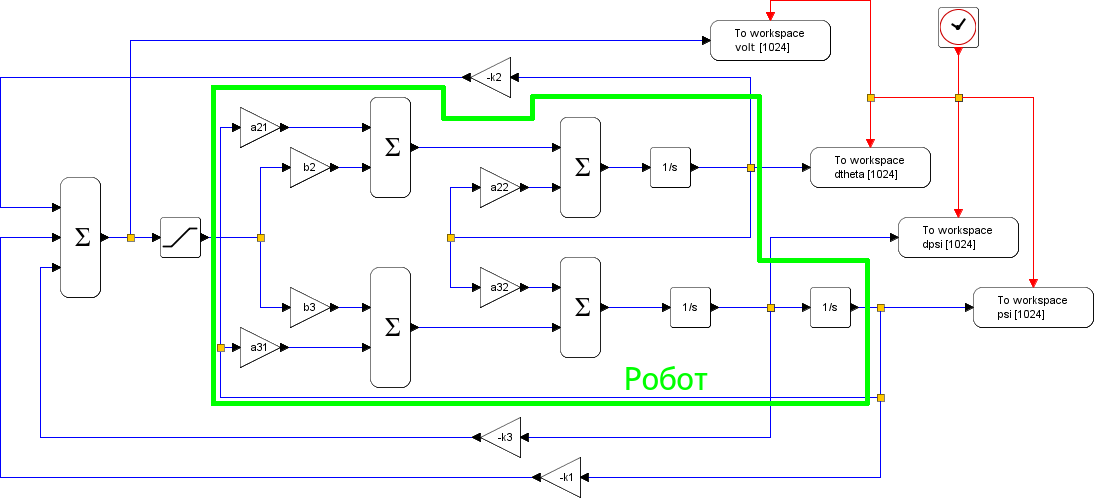
\includegraphics[width=\textwidth]{struct_sheme.png}}
	\caption{Схема моделирования.}
	\label{struct_sheme}
\end{figure}

Обратите внимание, различные каналы связи соединяются только в местах, помеченных оранжевыми квадратиками.
Величины k1, k2 и k3 есть соответствующие элементы матрицы~$K$.
Входящий в эту схему блок с рисунком ломаной, нужен ровно для того же, для чего он использовался в схеме из лабораторной~№3: он ограничивает поступающее на свой вход напряжение определенными границами: $-U_{max}$ и $U_{max}$. 

\newpage
\section{Цель работы}
\hspace*{\parindent}Получить опыт составления модели вход-состояние-выход для относительно сложного электромеханического устройства.
Познакомиться с понятием П-регулятора состояния, расчетом его коэффициентов и принципами работы неполноприводных роботов, находящихся под его управлением.

\section{Порядок выполнения работы}
\begin{enumerate}
	\item Соберите одного из роботов, рассмотренных в основной части пособия. Особое внимание при этом уделите 
	\begin{itemize}
	\item в случае работы с обратным маятником на тележке:
	\begin{itemize}
	\item строению крепежного узла, соединяющего маятник с тележкой: он должен включать в себя датчик HiTechnic Angle Sensor (см.~Приложение~\ref{append:angle_sensor});
	\item Приложению~\ref{append:inv_pend_constr}: в нем содержится пример конструкции исследуемого робота.
	\end{itemize}
	\item в случае работы с Segway:
	\begin{itemize}
	\item тому факту, что для определения значений величин $\psi$ и $\dot\psi$ Segway следует оборудовать датчиком HiTechnic Gyro Sensor (см.~Приложение~\ref{append:gyro_sensor}).
	\end{itemize}
	\end{itemize}	
	
	Также следует учесть следующее. 
	
	При построении математической модели механической системы на используемом для этого рисунке последняя показывается в том состоянии, которому соответствуют положительные значения обобщенных координат\lefteqn.\footnote{Достаточно очевидно, что обобщенные координаты могут принимать как положительные, так и отрицательные значения. Например, в случае c обратным маятником на тележке при отклонении первого из положения равновесия в одну сторону угол~$\psi$ будет б\'oльшим нуля, а в другую~--- меньшим нуля. То же можно сказать и про угол~$\theta$.} Из указанной причины следует, что отмеченные на рис.~5, 6 и 8 документа <<Лабораторная работа №5а~\dots Часть~1~\dots>> и на рис.~2 или~3 документа <<Лабораторная работа №5б~\dots Часть~1~\dots>> углы $\psi$ и $\theta$ положительны. Отсюда можно сделать вывод, что отсчет данных углов у конструируемого робота должен производится аналогичным образом. 
	
	\item Измерьте и/или рассчитайте все параметры робота, встречающиеся в его математической модели, например массу колес, длину маятника, и запишите получившиеся значения.
	
	Отдельно стоит отметить тот факт, что при расчете момента инерции <<тела>> Segway входящие в него командный блок, датчик HiTechnic Gyro Sensor и моторы NXT следует принять за однородные параллелепипеды (см.~рис.~\ref{paraps}\footnote{Момент инерции показанной на данном рисунке конструкции, относительно горизонтальной оси, проходящей через ее центр масс и перпендикулярной направлению движения робота, есть сумма моментов инерции относительно нее каждого из параллелепипедов. 
Напоминаем, что последние можно определить с помощью теоремы Штейнера	.}).
	
\begin{figure}[h]
	\noindent\centering{ 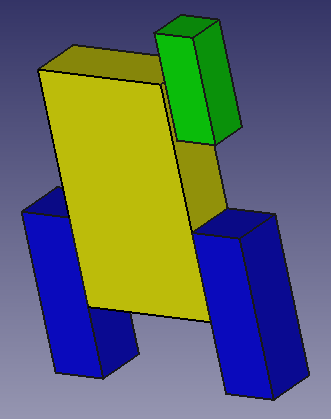
\includegraphics[scale=0.65]{paraps.png} }
	\caption{Аппроксимация <<тела>> Segway параллелепипедами.}
	\label{paraps}
\end{figure}
  
  	\item Сформируйте матрицу управляемости $Y$ и убедитесь, что ее определитель не равен нулю.
	\item Выберите некоторое значение для времени переходного процесса $t_\text{п}$ и рассчитайте коэффициенты П-регулятора состояния так, как это описано в основной части данного пособия.
	Учтите, что получающиеся в ходе расчетов коэффициенты в зависимости от своего физического смысла измеряются или в $\text{В}/\text{рад}$, или в $\text{В}\cdot\text{с}/\text{рад}$.
	\item Напишите для робота управляющую программу.
	В~ее основе должен лежать П-регулятор состояния, а следовательно должны использоваться найденные ранее коэффициенты.
	
	Также создаваемая программа должна снимать с робота и записывать в текстовый файл данные, достаточные для построения графиков, подобных показанным на рис.~\ref{fig:graphics_from_inv_pend} и~\ref{fig:graphics_from_segway}.
	
\begin{figure}[h]
	\noindent\centering{ 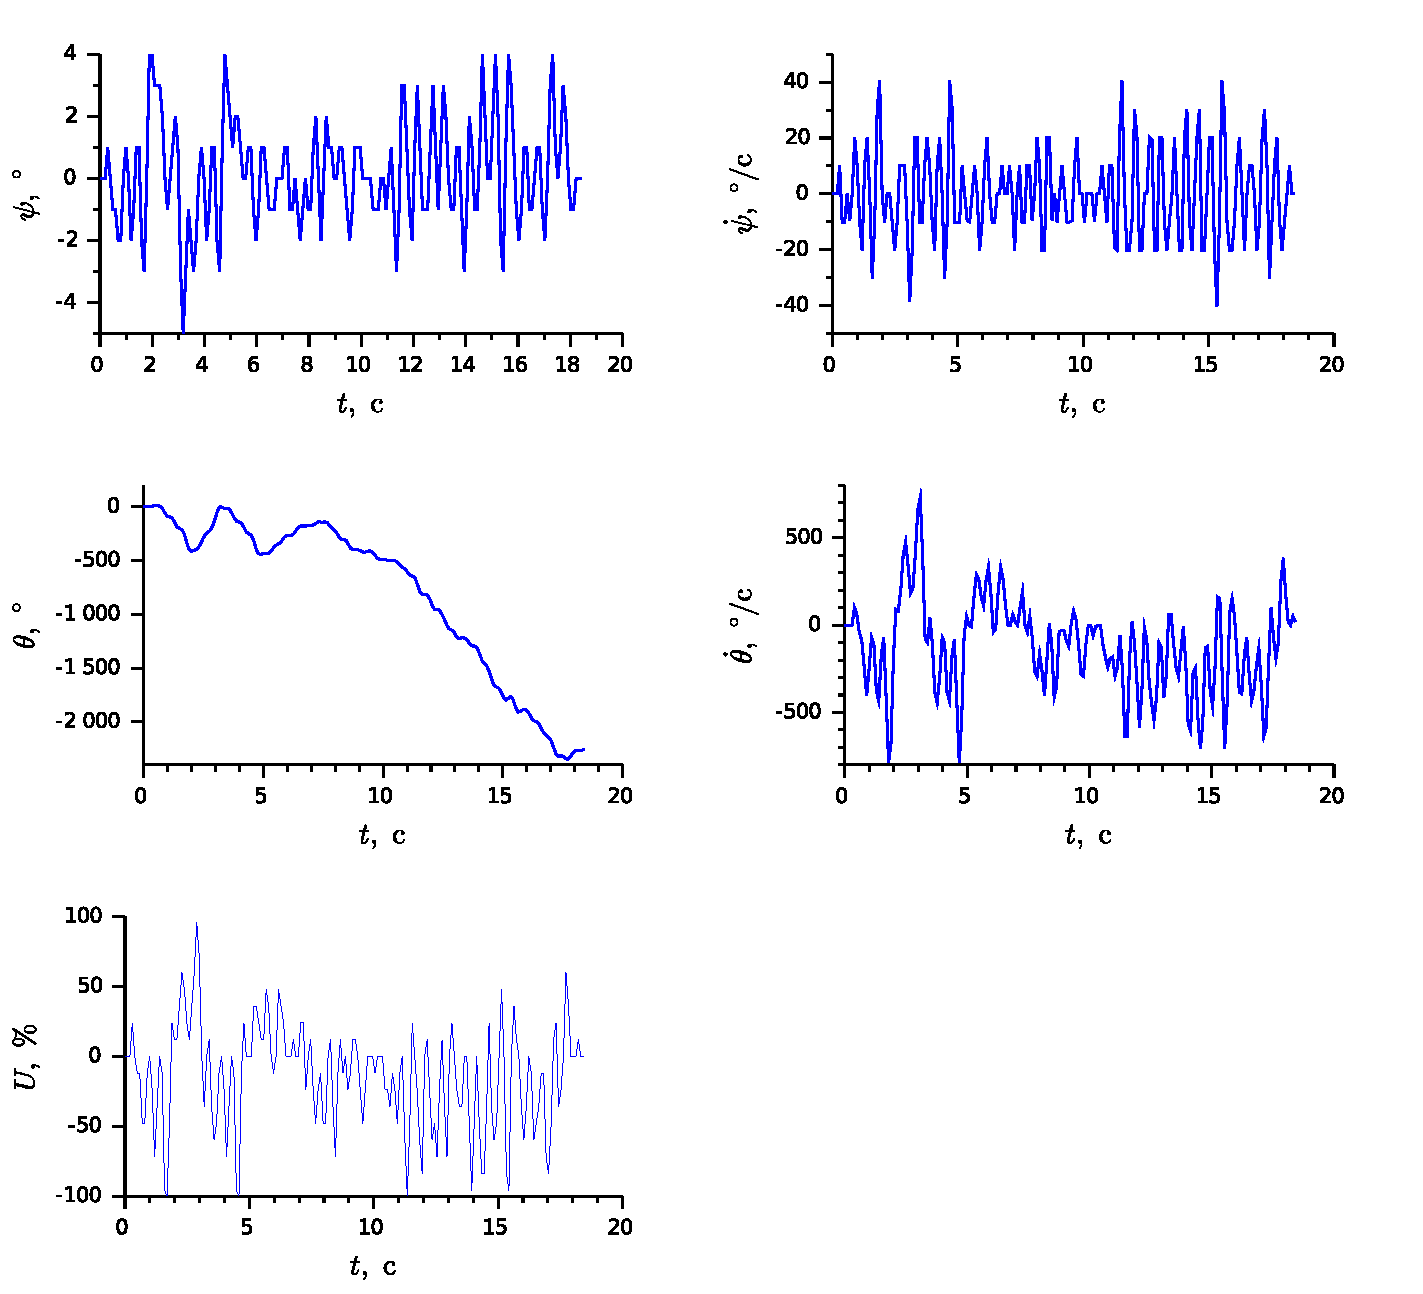
\includegraphics[width=\textwidth]{graphics_from_inv_pend.pdf} }
	\caption{Графики, построенные по данным, снятым с робота <<обратный маятник на тележке>>.}
	\label{fig:graphics_from_inv_pend}
\end{figure}

\begin{figure}[p]
	\noindent\centering{ 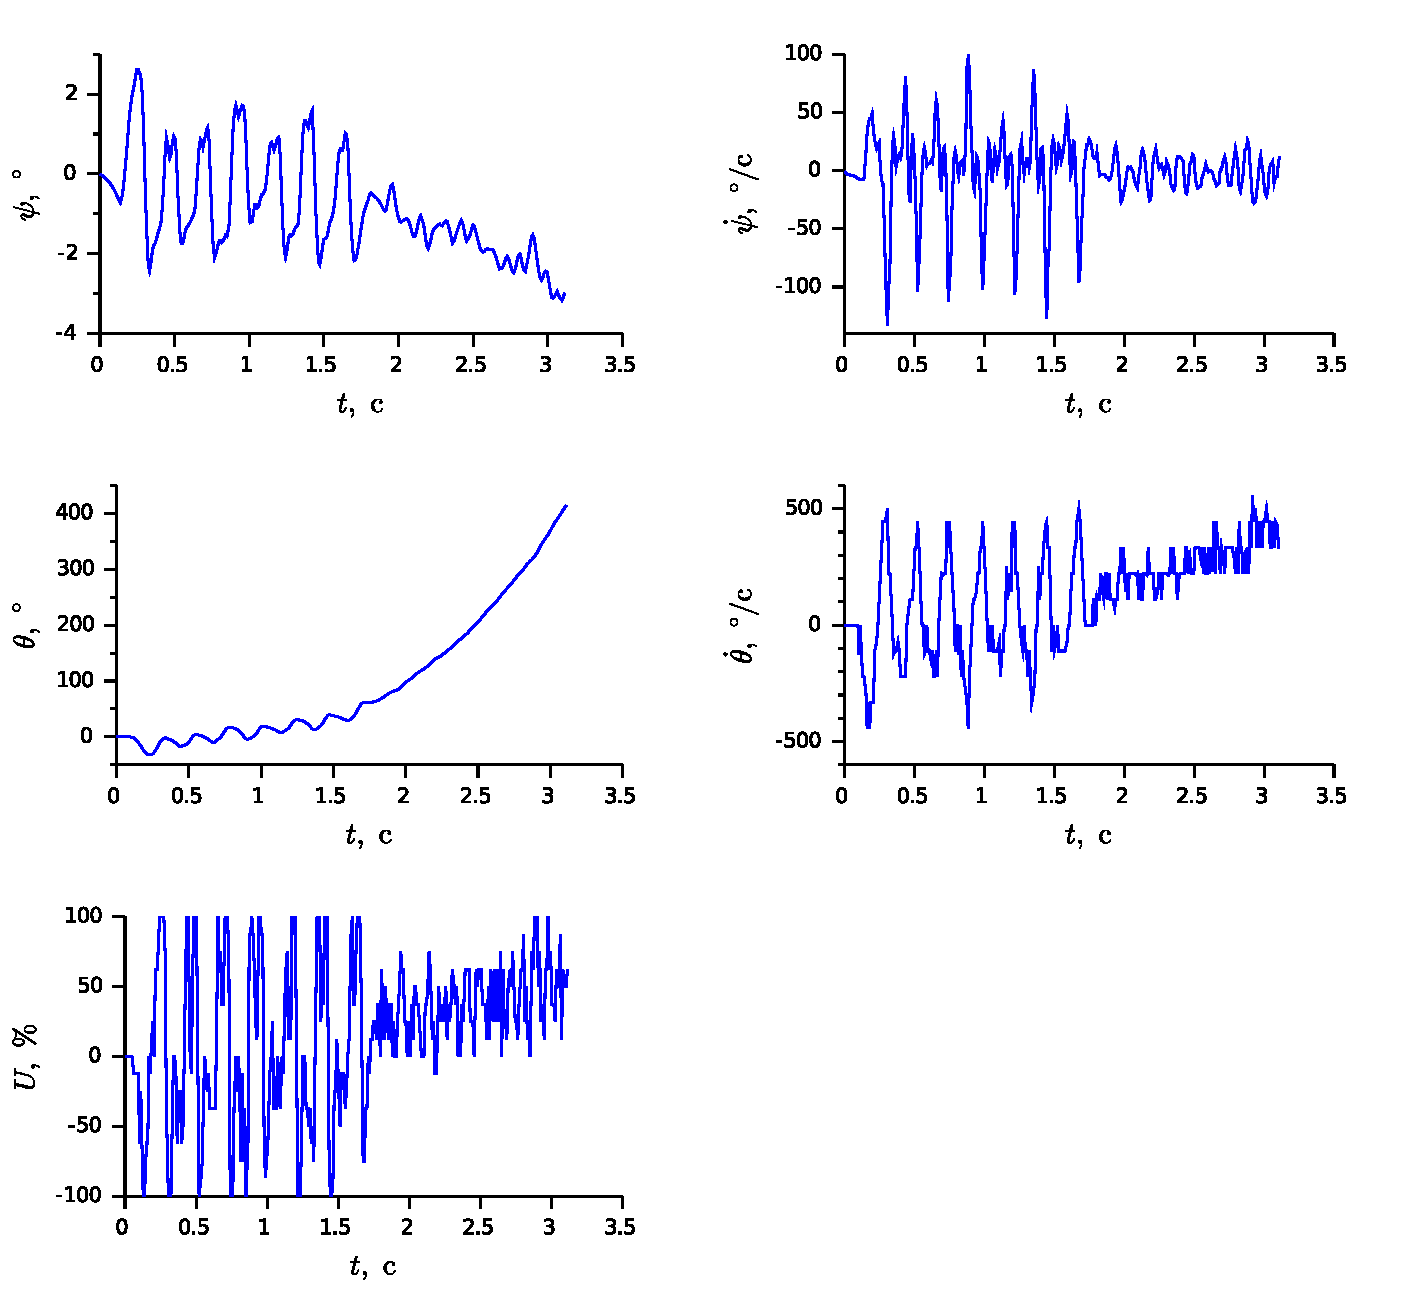
\includegraphics[width=\textwidth]{graphics_from_segway.pdf} }
	\caption{Графики, построенные по снятым с Segway данным.}
	\label{fig:graphics_from_segway}
\end{figure}

	\item Загрузите программу в командный блок и проверьте работоспособность робота.
	В~случае отрицательного результата измените время переходного процесса $t_\text{п}$ и повторите расчет со всеми последующими действиями.
	В~случае повторных неудач, продолжайте изменять время переходного процесса и заново проделывать все необходимые действия.
	\item Постройте в Xcos схему моделирования разрабатываемого робота. При работе над ней учтите, что значения полей Initial state у интеграторов в отличие от прошлых лабораторных работ не должны быть равными нулю. В~этот раз в них следует прописать название тех переменных (в каждый блок свою), в которых будут храниться начальные условия, например psi0, dpsi0, dtheta0. В~таком случае, если надо будет, например, исследовать поведение механизма при начальном отклонении покоящегося маятника на $\pi/12 \text{ рад}$ и покоящейся тележке, необходимо будет перед моделированием дать в Scilab команду: \verb|psi0=%pi/12, dpsi0=0, dtheta0=0|.
	\item Для трех наборов начальных условий~--- значений переменных dpsi0, dtheta0, psi0~--- промоделируйте исследуемый процесс и постройте соответствующие графики. Пример последних можно видеть на рис.~\ref{fig:graphics_from_model}.
\end{enumerate}

\begin{figure}[p]
	\noindent\centering{ 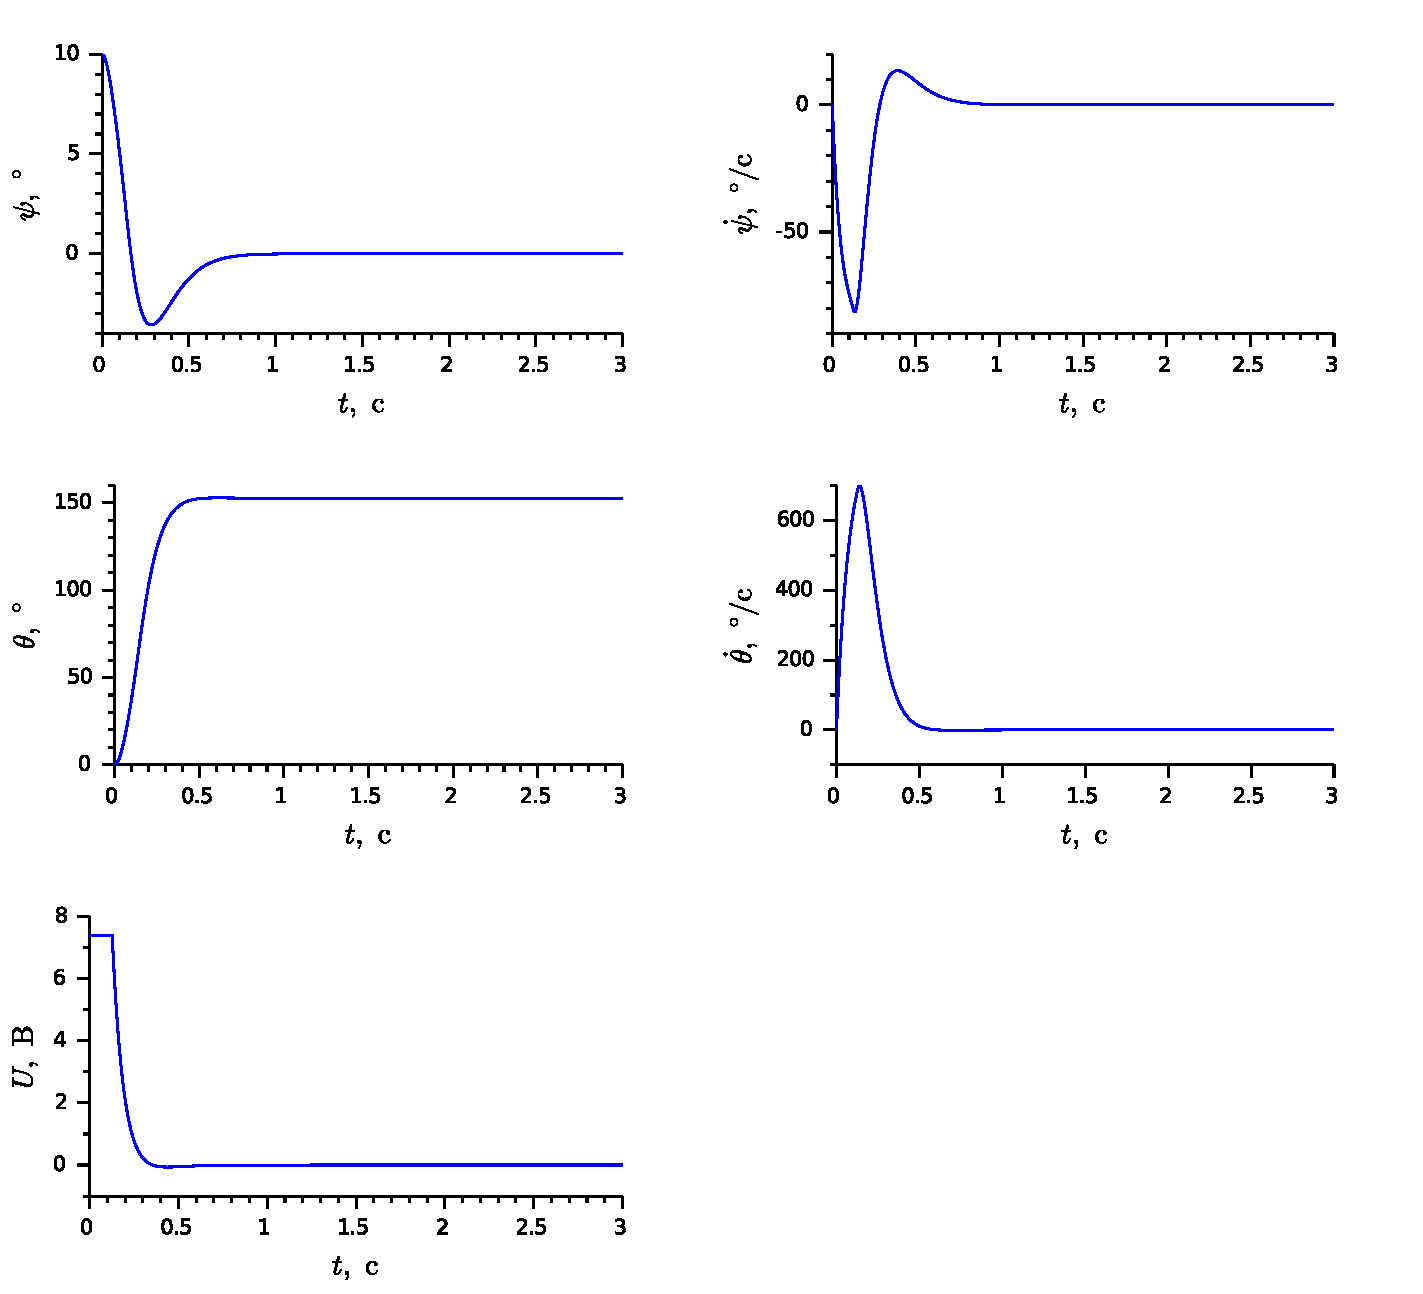
\includegraphics[width=\textwidth]{graphics_from_model.pdf} }
	\caption{Графики~--- результаты моделирования соответствующей схемы.}
	\label{fig:graphics_from_model}
\end{figure}

\section{Содержание отчета}
\begin{enumerate}
\item Результаты всех измерений, графики и вычисления, предусмотренных(ые) разделом <<Порядок выполнения работы>>.
\item Фотография робота (в том случае, если его конструкция сильно отличается от приведенных в пособии ее примеров).
\item Построенная в Xcos схема моделирования (аналогичная представленной на рис.~\ref{struct_sheme}).
\item Исходный код программы робота.
\item Исходные коды расчетных программ для Scilab.
\item Выводы о проделанной работе.
\end{enumerate}

\newpage
\section*{Приложение~\myappnum\label{append:some_maths}\\
Вычисление характеристического полинома матрицы $F$ и получение дифференциальных уравнений относительно функций $\psi(t)$ и $\theta(t)$}
\paragraph*{Характеристический полином матрицы $F$}$\phantom{-}$\\
\hspace*{\parindent}Вычисляя характеристический полином матрицы $F$ можно получить следующее:
\begin{multline}
\det(\lambda E - F) = 
\det\left(\begin{bmatrix}
\lambda & 0       & 0\\
0       & \lambda & 0\\
0       & 0       & \lambda
\end{bmatrix}
-
\begin{bmatrix}
0      & 0      & 1\\
f_{21} & f_{22} & f_{23}\\
f_{31} & f_{32} & f_{33}
\end{bmatrix}\right) = 
\begin{vmatrix}
\lambda      & 0                & -1\\
-f_{21}      & \lambda - f_{22} & -f_{23}\\
-f_{31}      & -f_{32}          & \lambda - f_{33}
\end{vmatrix} = \\
=
\lambda
\begin{vmatrix}
\lambda - f_{22} & -f_{23}\\
-f_{32}          & \lambda - f_{33}
\end{vmatrix}
-
\begin{vmatrix}
-f_{21}      & \lambda - f_{22}\\
-f_{31}      & -f_{32}
\end{vmatrix} = 
\lambda((\lambda - f_{22})(\lambda - f_{33}) - f_{23}f_{32}) - (f_{21}f_{32}+\\+f_{31}(\lambda - f_{22})) = \lambda^3 - (f_{22}+f_{33})\lambda^2 + (f_{22}f_{33} - f_{23}f_{32} - f_{31})\lambda + (f_{22}f_{31} - f_{21}f_{32})\ldotp
\end{multline}

\paragraph*{Дифференциальное уравнение относительно функции $\psi(t)$}$\phantom{-}$\\
\hspace*{\parindent}Согласно уравнению~\eqref{eq:dx_Fx} справедливо
\begin{equation}
\begin{bmatrix}
\dot\psi \\ \ddot\theta \\ \ddot\psi
\end{bmatrix}
=
\begin{bmatrix}
0      & 0      & 1\\
f_{21} & f_{22} & f_{23}\\
f_{31} & f_{32} & f_{33}
\end{bmatrix}
\begin{bmatrix}
\psi \\ \dot\theta \\ \dot\psi
\end{bmatrix}\!\!\ldotp
\end{equation}
Данное выражение можно переписать как
\begin{equation}\label{eq:system_with_F}
	\left\{
	\begin{aligned}
		\!&\dot\psi = \dot\psi \\
		\!&\ddot\theta = f_{21}\psi + f_{22}\dot\theta + f_{23}\dot\psi\\
		\!&\ddot\psi = f_{31}\psi + f_{32}\dot\theta + f_{33}\dot\psi\ldotp
	\end{aligned}
	\right.
\end{equation}

Дифференцируя последнее уравнение, можно получить следующее:
\begin{equation}\label{eq:eq_for_dddot_psi}
\dddot\psi = f_{31}\dot\psi + f_{32}\ddot\theta + f_{33}\ddot\psi,
\end{equation}
из него же следует то, что
\begin{equation}\label{eq:eq_for_dot_theta}
f_{32}\dot\theta = \ddot\psi - f_{31}\psi - f_{33}\dot\psi\ldotp
\end{equation}

С~учетом второго уравнения системы~\eqref{eq:system_with_F} выражение~\eqref{eq:eq_for_dddot_psi} примет вид:
\begin{equation}
\dddot\psi = f_{31}\dot\psi + f_{32}f_{21}\psi + f_{32}f_{22}\dot\theta + f_{32}f_{23}\dot\psi + f_{33}\ddot\psi,
\end{equation}
данное же выражение с учетом~\eqref{eq:eq_for_dot_theta} преобразуется до следующего дифференциального уравнения:
\begin{gather}
\dddot\psi = f_{31}\dot\psi + f_{32}f_{21}\psi + f_{22}\ddot\psi - f_{22}f_{31}\psi - f_{22}f_{33}\dot\psi + f_{32}f_{23}\dot\psi + f_{33}\ddot\psi\\
\dddot\psi - (f_{22}+f_{33})\ddot\psi + (f_{22}f_{33}-f_{32}f_{23}-f_{31})\dot\psi + (f_{22}f_{31} - f_{32}f_{21})\psi = 0
\end{gather}

\paragraph*{Дифференциальное уравнение относительно функции $\omega(t)$}$\phantom{-}$\\
\hspace*{\parindent}С~учетом того, что $\omega = \dot\theta$, два последних уравнения системы~\eqref{eq:system_with_F} можно переписать так:
\begin{equation}\label{eq:two_eqs_with_omega_not_theta}
	\left\{
	\begin{aligned}
		\!&\dot\omega = f_{21}\psi + f_{22}\omega + f_{23}\dot\psi\\
		\!&\ddot\psi = f_{31}\psi + f_{32}\omega + f_{33}\dot\psi\ldotp
	\end{aligned}
	\right.
\end{equation}
Взяв от полученных выражений несколько производных можно получить следующую систему:
\begin{equation}
\left\{
	\begin{aligned}
		\!&\dot\omega = f_{21}\psi + f_{22}\omega + f_{23}\dot\psi\\
		\!&\ddot\omega = f_{21}\dot\psi + f_{22}\dot\omega + f_{23}\ddot\psi\\
		\!&\dddot\omega = f_{21}\ddot\psi + f_{22}\ddot\omega + f_{23}\dddot\psi\\		
		\!&\ddot\psi = f_{31}\psi + f_{32}\omega + f_{33}\dot\psi\\
		\!&\dddot\psi = f_{31}\dot\psi + f_{32}\dot\omega + f_{33}\ddot\psi\ldotp
	\end{aligned}
\right.\qquad\Rightarrow\qquad
\left\{
	\begin{aligned}
		\!&\dot\omega - f_{22}\omega = f_{21}\psi + f_{23}\dot\psi\\
		\!&\ddot\omega - f_{22}\dot\omega = f_{21}\dot\psi + f_{23}\ddot\psi\\
		\!&- f_{22}\ddot\omega = -\dddot\omega + f_{21}\ddot\psi + f_{23}\dddot\psi\\		
		\!&- f_{32}\omega = f_{31}\psi + f_{33}\dot\psi - \ddot\psi\\
		\!&- f_{32}\dot\omega = f_{31}\dot\psi + f_{33}\ddot\psi - \dddot\psi\ldotp
	\end{aligned}
\right.
\end{equation}
матричное представление которой имеет вид
\begin{equation}
\begin{bmatrix}
-f_{22} & 1       & 0\\
0       & -f_{22} & 1\\
0       & 0       & -f_{22}\\
-f_{32} & 0       & 0\\
0       & -f_{32} & 0
\end{bmatrix}
\begin{bmatrix}
\omega \\ \dot\omega \\ \ddot\omega
\end{bmatrix}
=
\begin{bmatrix}
0  & f_{21} & f_{23} & 0      & 0\\
0  & 0      & f_{21} & f_{23} & 0\\
-1 & 0      & 0      & f_{21} & f_{23}\\
0  & f_{31} & f_{33} & -1     & 0\\
0  & 0      & f_{31} & f_{33} & -1
\end{bmatrix}
\begin{bmatrix}
\dddot\omega \\ \psi \\ \dot\psi \\ \ddot\psi \\ \dddot\psi
\end{bmatrix}\!\!\ldotp
\end{equation} 

Произведя некоторые вычисления\footnote{Часть одной из ниже следующих матриц, которая для краткости записи была опущена, легко можно узнать, выполнив, например, в Maxima следующие команды:\\
\texttt{M:matrix([-f22,1,0],[0,-f22,1],[0,0,-f22],[-f32,0,0],[0,-f32,0]);}\\
\texttt{P:matrix([0,f21,f23,0,0],[0,0,f21,f23,0],[-1,0,0,f21,f23],[0,f31,f33,-1,0],[0,0,f31,f33,-1]);}\\
\texttt{ratsimp(invert(P).M);}}:
\begin{gather}
\begin{bmatrix}
\dddot\omega \\ \psi \\ \dot\psi \\ \ddot\psi \\ \dddot\psi
\end{bmatrix}
=
\begin{bmatrix}
0  & f_{21} & f_{23} & 0      & 0\\
0  & 0      & f_{21} & f_{23} & 0\\
-1 & 0      & 0      & f_{21} & f_{23}\\
0  & f_{31} & f_{33} & -1     & 0\\
0  & 0      & f_{31} & f_{33} & -1
\end{bmatrix}^{-1}
\begin{bmatrix}
-f_{22} & 1       & 0\\
0       & -f_{22} & 1\\
0       & 0       & -f_{22}\\
-f_{32} & 0       & 0\\
0       & -f_{32} & 0
\end{bmatrix}
\begin{bmatrix}
\omega \\ \dot\omega \\ \ddot\omega
\end{bmatrix}\!\!,\\
%
\begin{bmatrix}
\dddot\omega \\ \psi \\ \dot\psi \\ \ddot\psi \\ \dddot\psi
\end{bmatrix}
=
\begin{bmatrix}
f_{21}f_{32}-f_{22}f_{31} & -f_{22}f_{33} + f_{23}f_{32} + f_{31} & f_{22}+f_{33}\\
\dots & \dots & \dots\\
\dots & \dots & \dots\\
\dots & \dots & \dots\\
\dots & \dots & \dots\\
\dots & \dots & \dots
\end{bmatrix}
\begin{bmatrix}
\omega \\ \dot\omega \\ \ddot\omega
\end{bmatrix}\!\!,
\end{gather}
для функции $\omega(t)$ можно получить следующее дифференциальное уравнение:
\begin{gather}
\dddot\omega = (f_{21}f_{32} - f_{22}f_{31})\omega - (f_{22}f_{33}-f_{23}f_{32}-f_{31})\dot\omega  + (f_{22}+f_{33})\ddot\omega\\
\dddot\omega - (f_{22}+f_{33})\ddot\omega + (f_{22}f_{33}-f_{23}f_{32}-f_{31})\dot\omega + (f_{22}f_{31} - f_{32}f_{21})\omega = 0
\end{gather}

\newpage
\section*{Приложение~\myappnum\label{append:angle_sensor}\\
Основы работы с датчиком HiTechnic Angle Sensor}
\hspace*{\parindent}HiTechnic Angle Sensor представляет из себя датчик, измеряющий разные количественные характеристики, описывающие вращение собственного <<ротора>>.
Под последним подразумевается его подвижная часть.

\begin{figure}[h]
	\noindent\centering{ 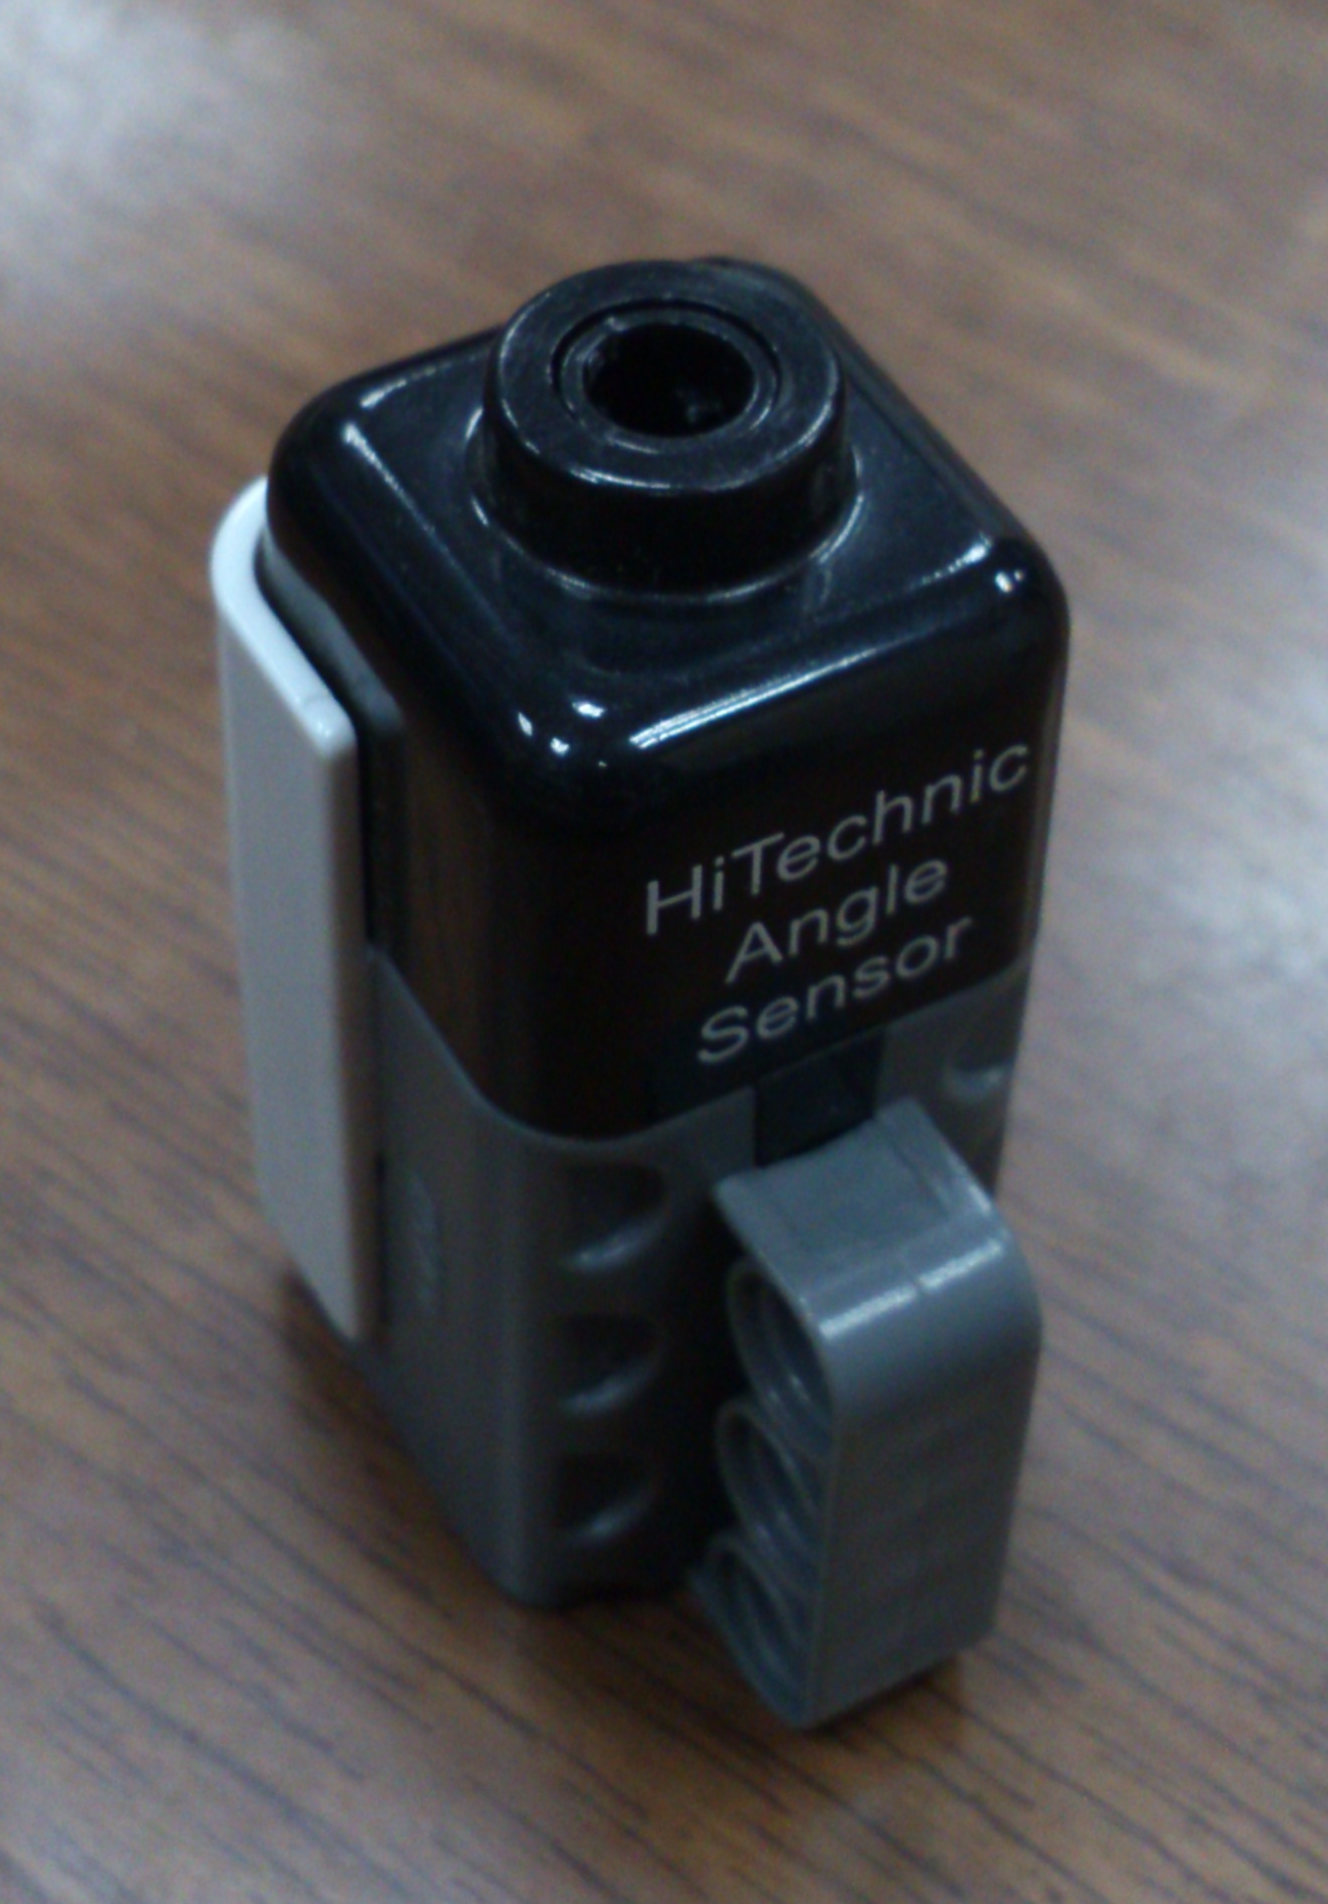
\includegraphics[scale=0.13]{sensor.png} }
	\caption{Общий вид датчика.}
	\label{sensor}
\end{figure}

Чтобы подключить этот датчик к программе, написанной на языке NXC, в нее необходимо добавить функцию \verb|SetSensorLowspeed(sensor_port)|.
Ее единственный аргумент~--- номер порта, к которому датчик подключен.

Считывание данных производится функцией \verb|ReadSensorHTAngle(sensor_port, abs_angle,| \verb|alg_angle, rpm)|.
В результате своего вызова она возвращает с датчика, подключенного в порт sensor\_port, три значения (по порядку): угловую координату (в градусах) текущего положения <<ротора>>, представляющую собой число от $0$ до $360$; угол отклонения (в градусах) от некоторого положения, представляющий из себя целое число, лежащее в диапазоне $(-2147483648;\ 2147483647)$; угловую скорость (в $\text{об}/\text{мин}$) вращения <<ротора>>~--- целое число, принадлежащее интервалу $(-1000;\ 1000)$.

В ряде случаев появляется необходимость обнулить (сбросить) текущие показание датчика.
Сделать это можно с помощью функции \verb|ResetSensorHTАngle(sensor_port, mode)|, причем значение последнего ее аргумента, являющего из себя целочисленную константу, следует принять равным макросу \verb|HTANGLE_MODE_CALIBRATE|, если надо обнулить обе величины abs\_angle и alg\_angle, а равным макросу \verb|HTANGLE_MODE_RESET|, если надо сбросить только alg\_angle.

Например, в приведенном ниже тексте некоторой программы с датчика (у которого все показания были предварительно обнулены), подключенного в порт~№2, снимаются выше указанные данные, и их значения записываются в переменные p1, p2 и p3:
\begin{verbatim}
task main(){	
    int p1, p3;
    long p2;
    ...
    SetSensorLowspeed(S2);
    ResetSensorHTАngle(S2, HTANGLE_MODE_CALIBRATE);
    ...
    ReadSensorHTAngle(S2, p1, p2, p3);
    ...
}	
\end{verbatim} 

\section*{Приложение~\myappnum\label{append:gyro_sensor}\\
Основы работы с датчиком HiTechnic Gyro Sensor}
\hspace*{\parindent}HiTechnic Gyro Sensor представляет из себя модуль, изображенный на рис.~\ref{sensor}. 
Этот датчик возвращает значение собственной угловой скорости вращения относительно оси, перпендикулярной той его поверхности, которая обращена <<к нам>> на рис.~\ref{sensor}б.
Данный факт пояснен красной стрелкой, показанной там же.

\begin{figure}[h]
	\begin{minipage}[h]{0.49\linewidth}
		\center{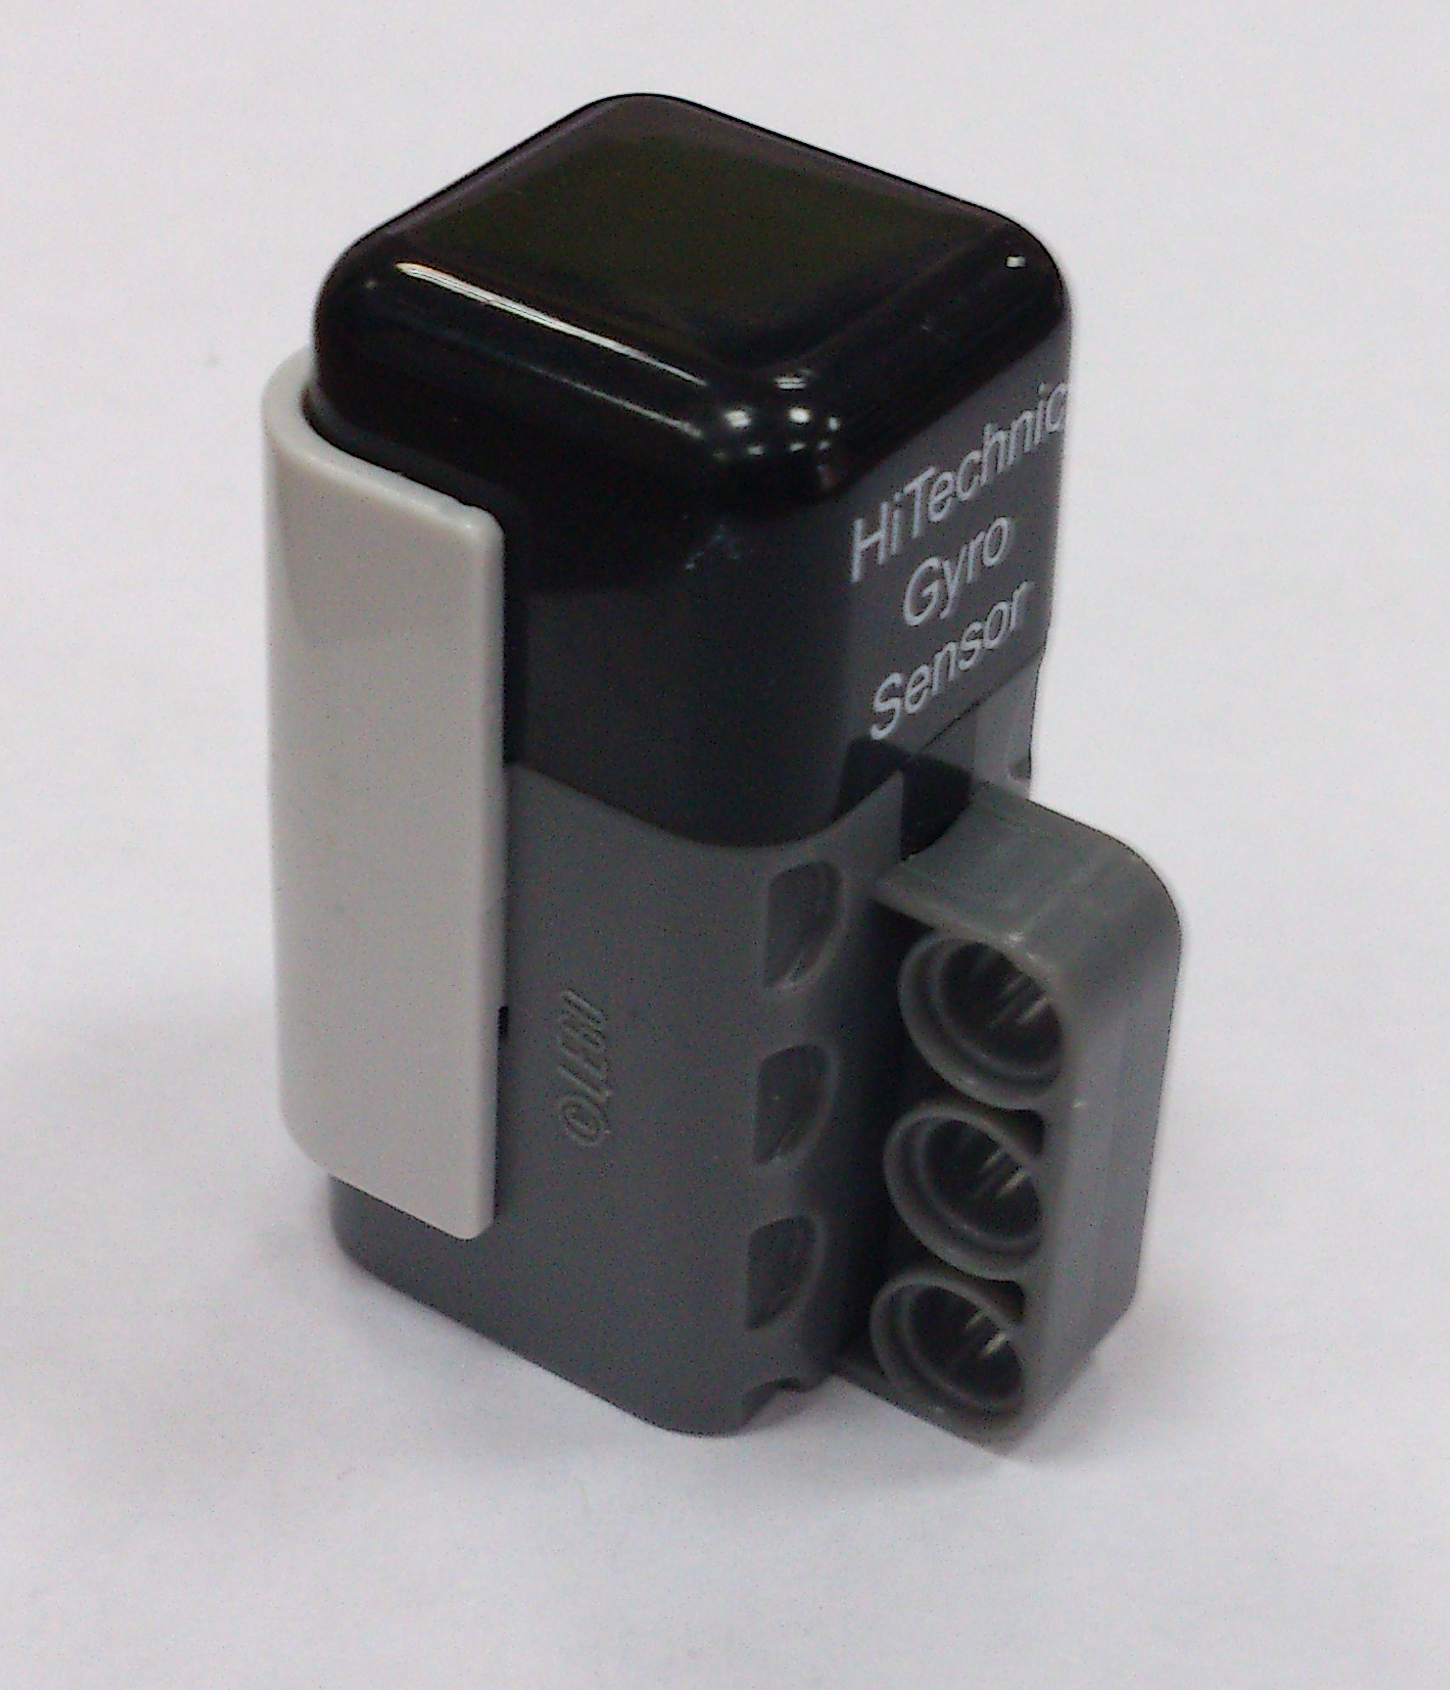
\includegraphics[height = 5.5 cm]{sensor_main.png} \\ а)}
	\end{minipage}
	\hfill
	\begin{minipage}[h]{0.49\linewidth}
		\center{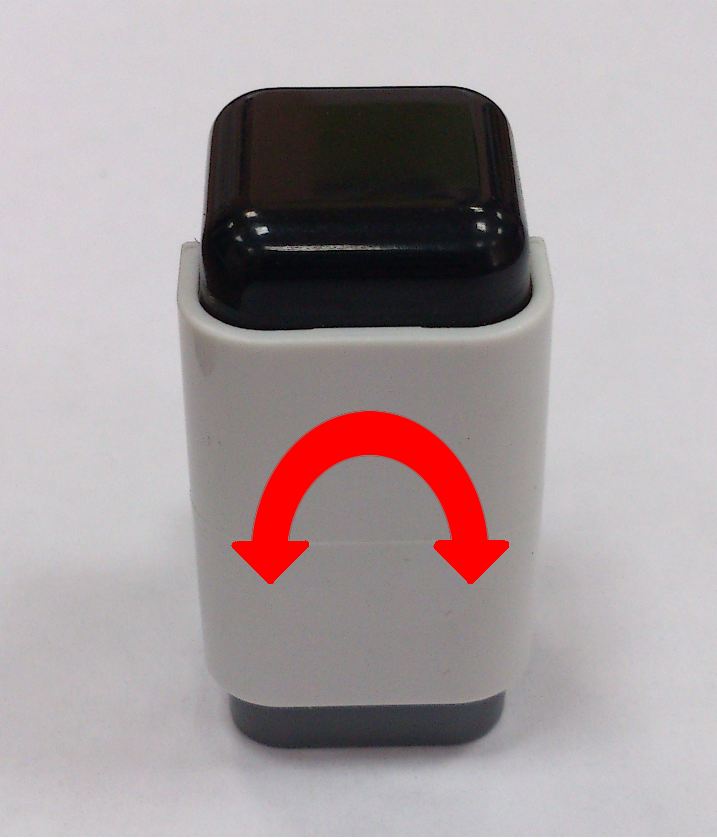
\includegraphics[height = 5.5 cm]{sensor_add.png} \\ б)}
	\end{minipage}
	\caption{Внешний вид NXT Gyro Sensor.}
	\label{sensor}
\end{figure}

Чтобы зарегистрировать NXT Gyro Sensor в исполняемой программе, в ее состав необходимо добавить функцию \verb|SetSensorHTGyro(sensor_port)|, чей единственный аргумент, как несложно догадаться, есть номер порта, в который этот датчик подключен.

Считывание данных производится функцией \verb|SensorHTGyro(sensor_port)|.
Возвращаемое ею целое значение представляет собой уже упомянутую угловую скорость, выраженную в [градусах в секунду].   
Знак получаемого числа определяется направлением вращения.

Особое внимание при работе с этим датчиком следует уделить тому, что в его данных может содержаться определенная ошибка, поэтому прежде, чем использовать сенсор в составе рабочего устройства, его необходимо дополнительно проверить. 
В случае, если указанная погрешность присутствует и носит простейший характер\lefteqn,\footnote{Например, датчик постоянно возвращает значение скорости на $n$ (градусов/с) меньшее или большее настоящего.} очевидно, что ее следует учесть, внеся определенные изменения в текст исполняемой роботом программы.

\newpage
\section*{Приложение \myappnum\label{append:inv_pend_constr}\\
Пример конструкции робота, называемого <<обратным маятником на тележке>>}
\hspace*{\parindent}Одну из возможных конструкций робота под названием <<обратный маятник на тележке>> описывают рис.~\ref{fig:first_pict_in_constr_example}~--\ref{fig:last_pict_in_constr_example}.
\vfill
\begin{figure}[h]
	\begin{minipage}[h]{0.49\linewidth}
		\center{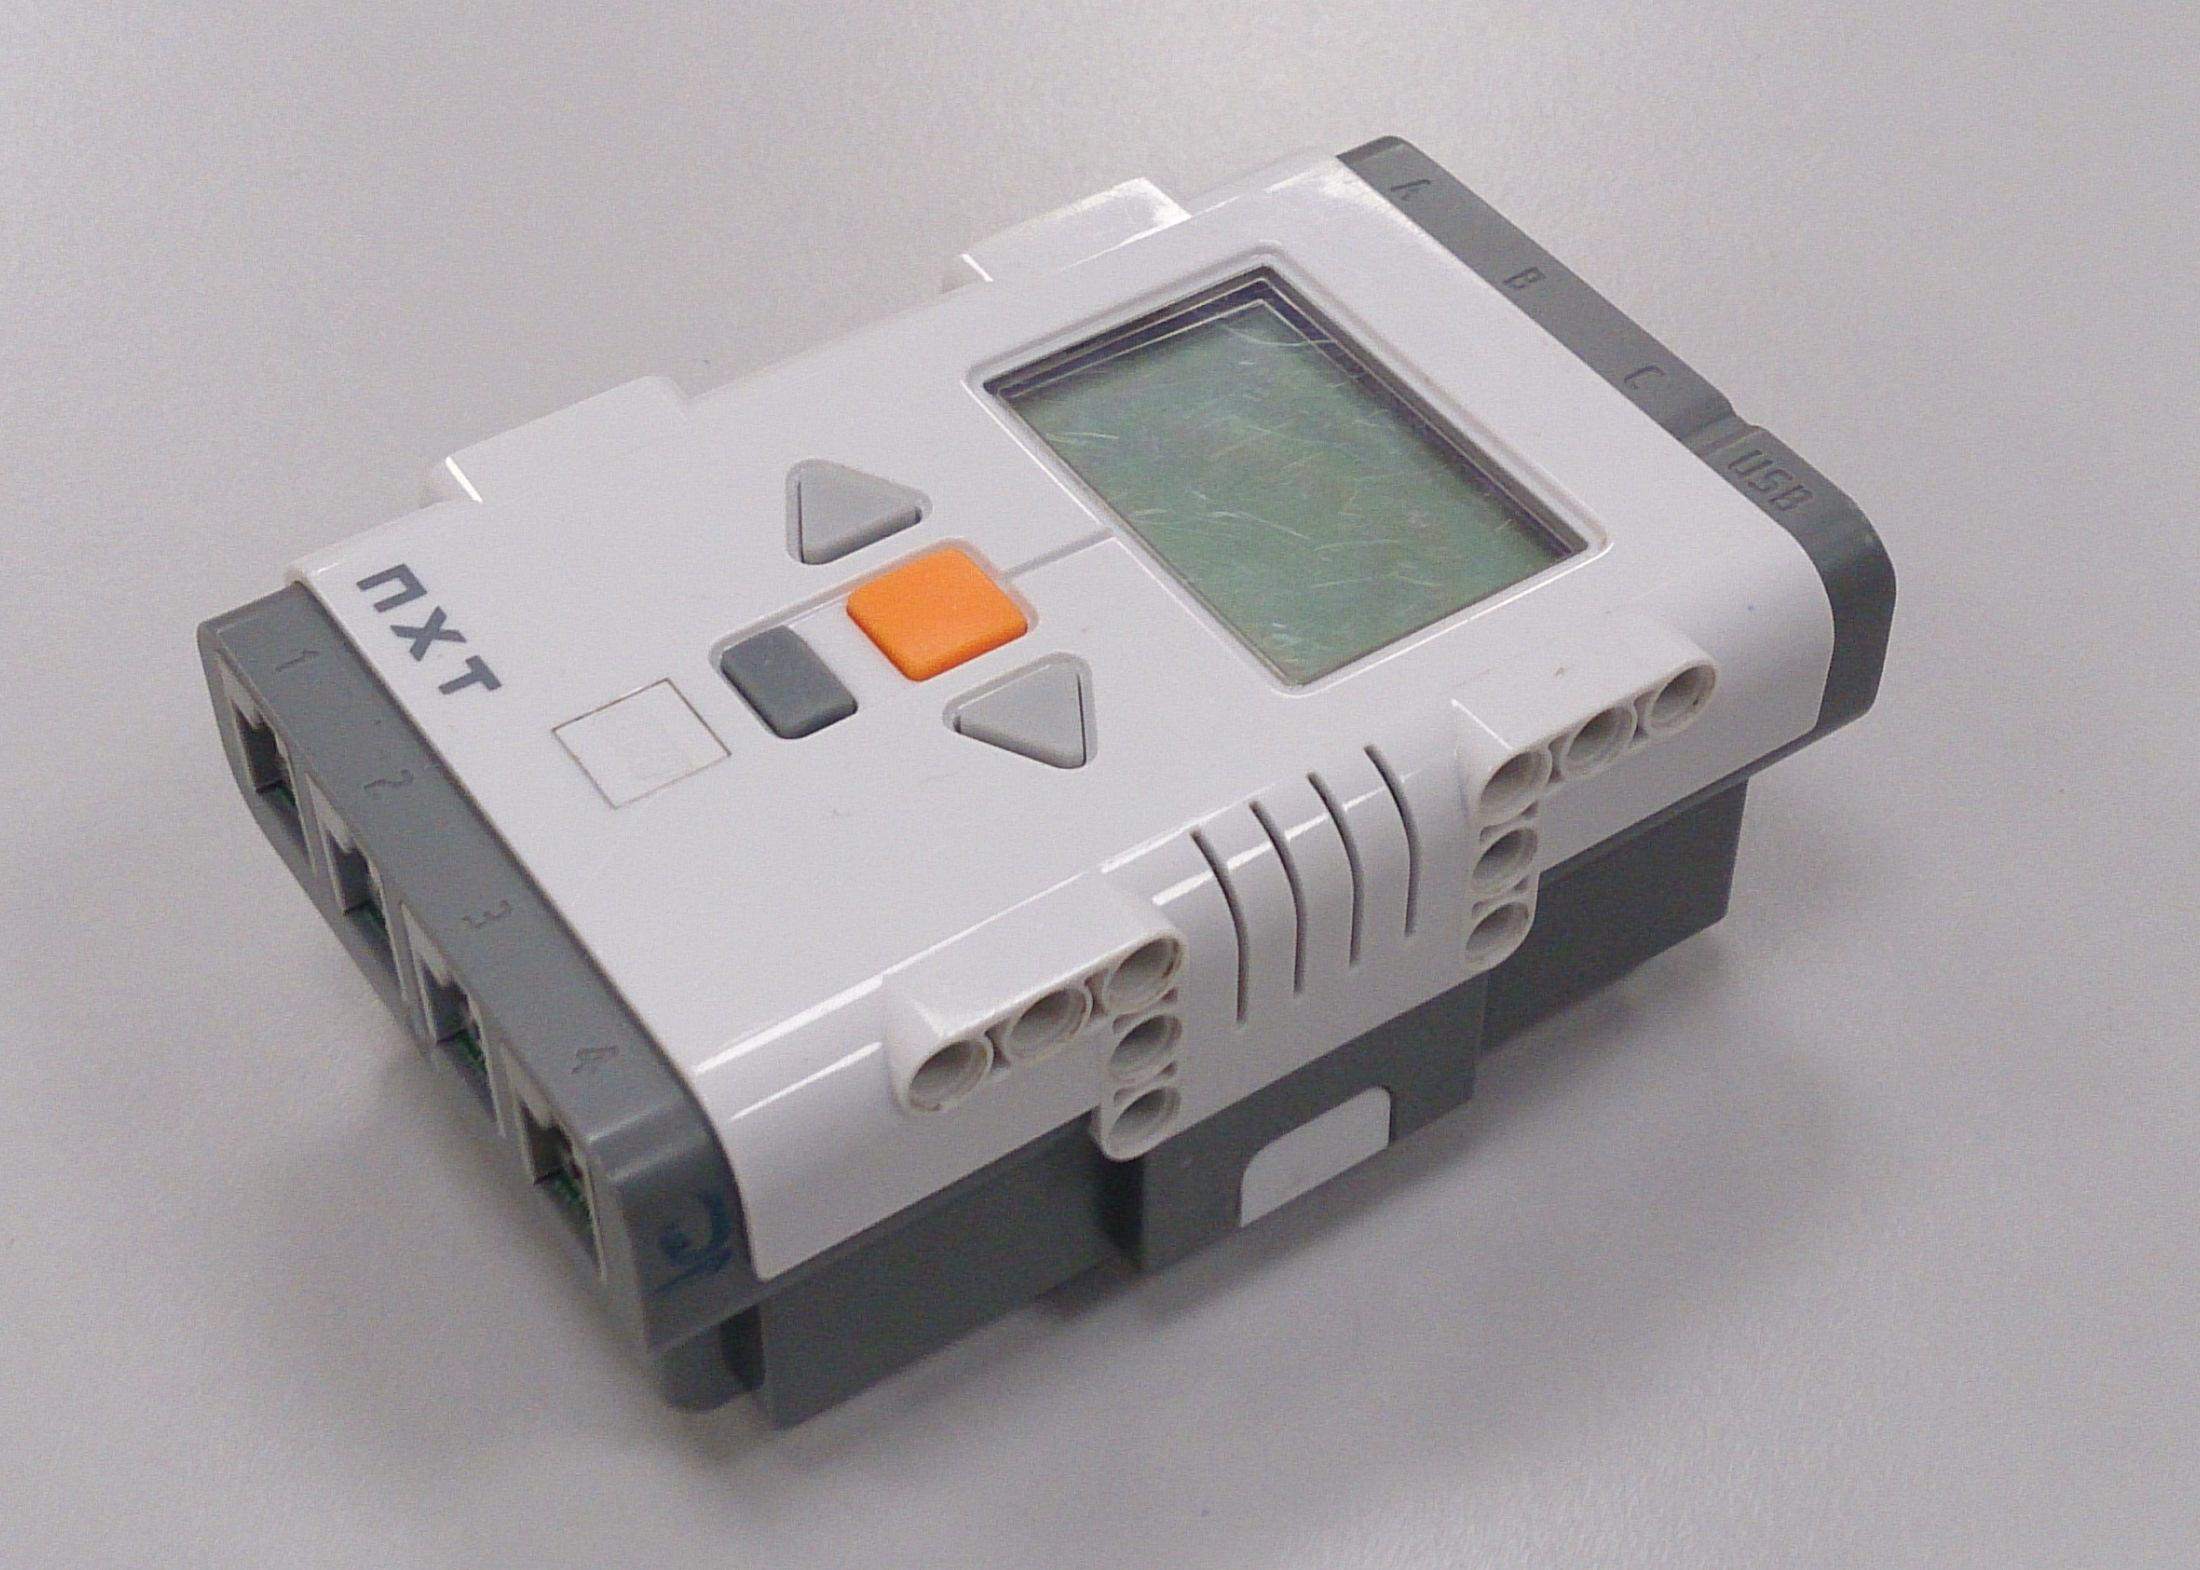
\includegraphics[height = 5.5 cm]{first.jpg} \\ а)}
	\end{minipage}
	\hfill
	\begin{minipage}[h]{0.49\linewidth}
		\center{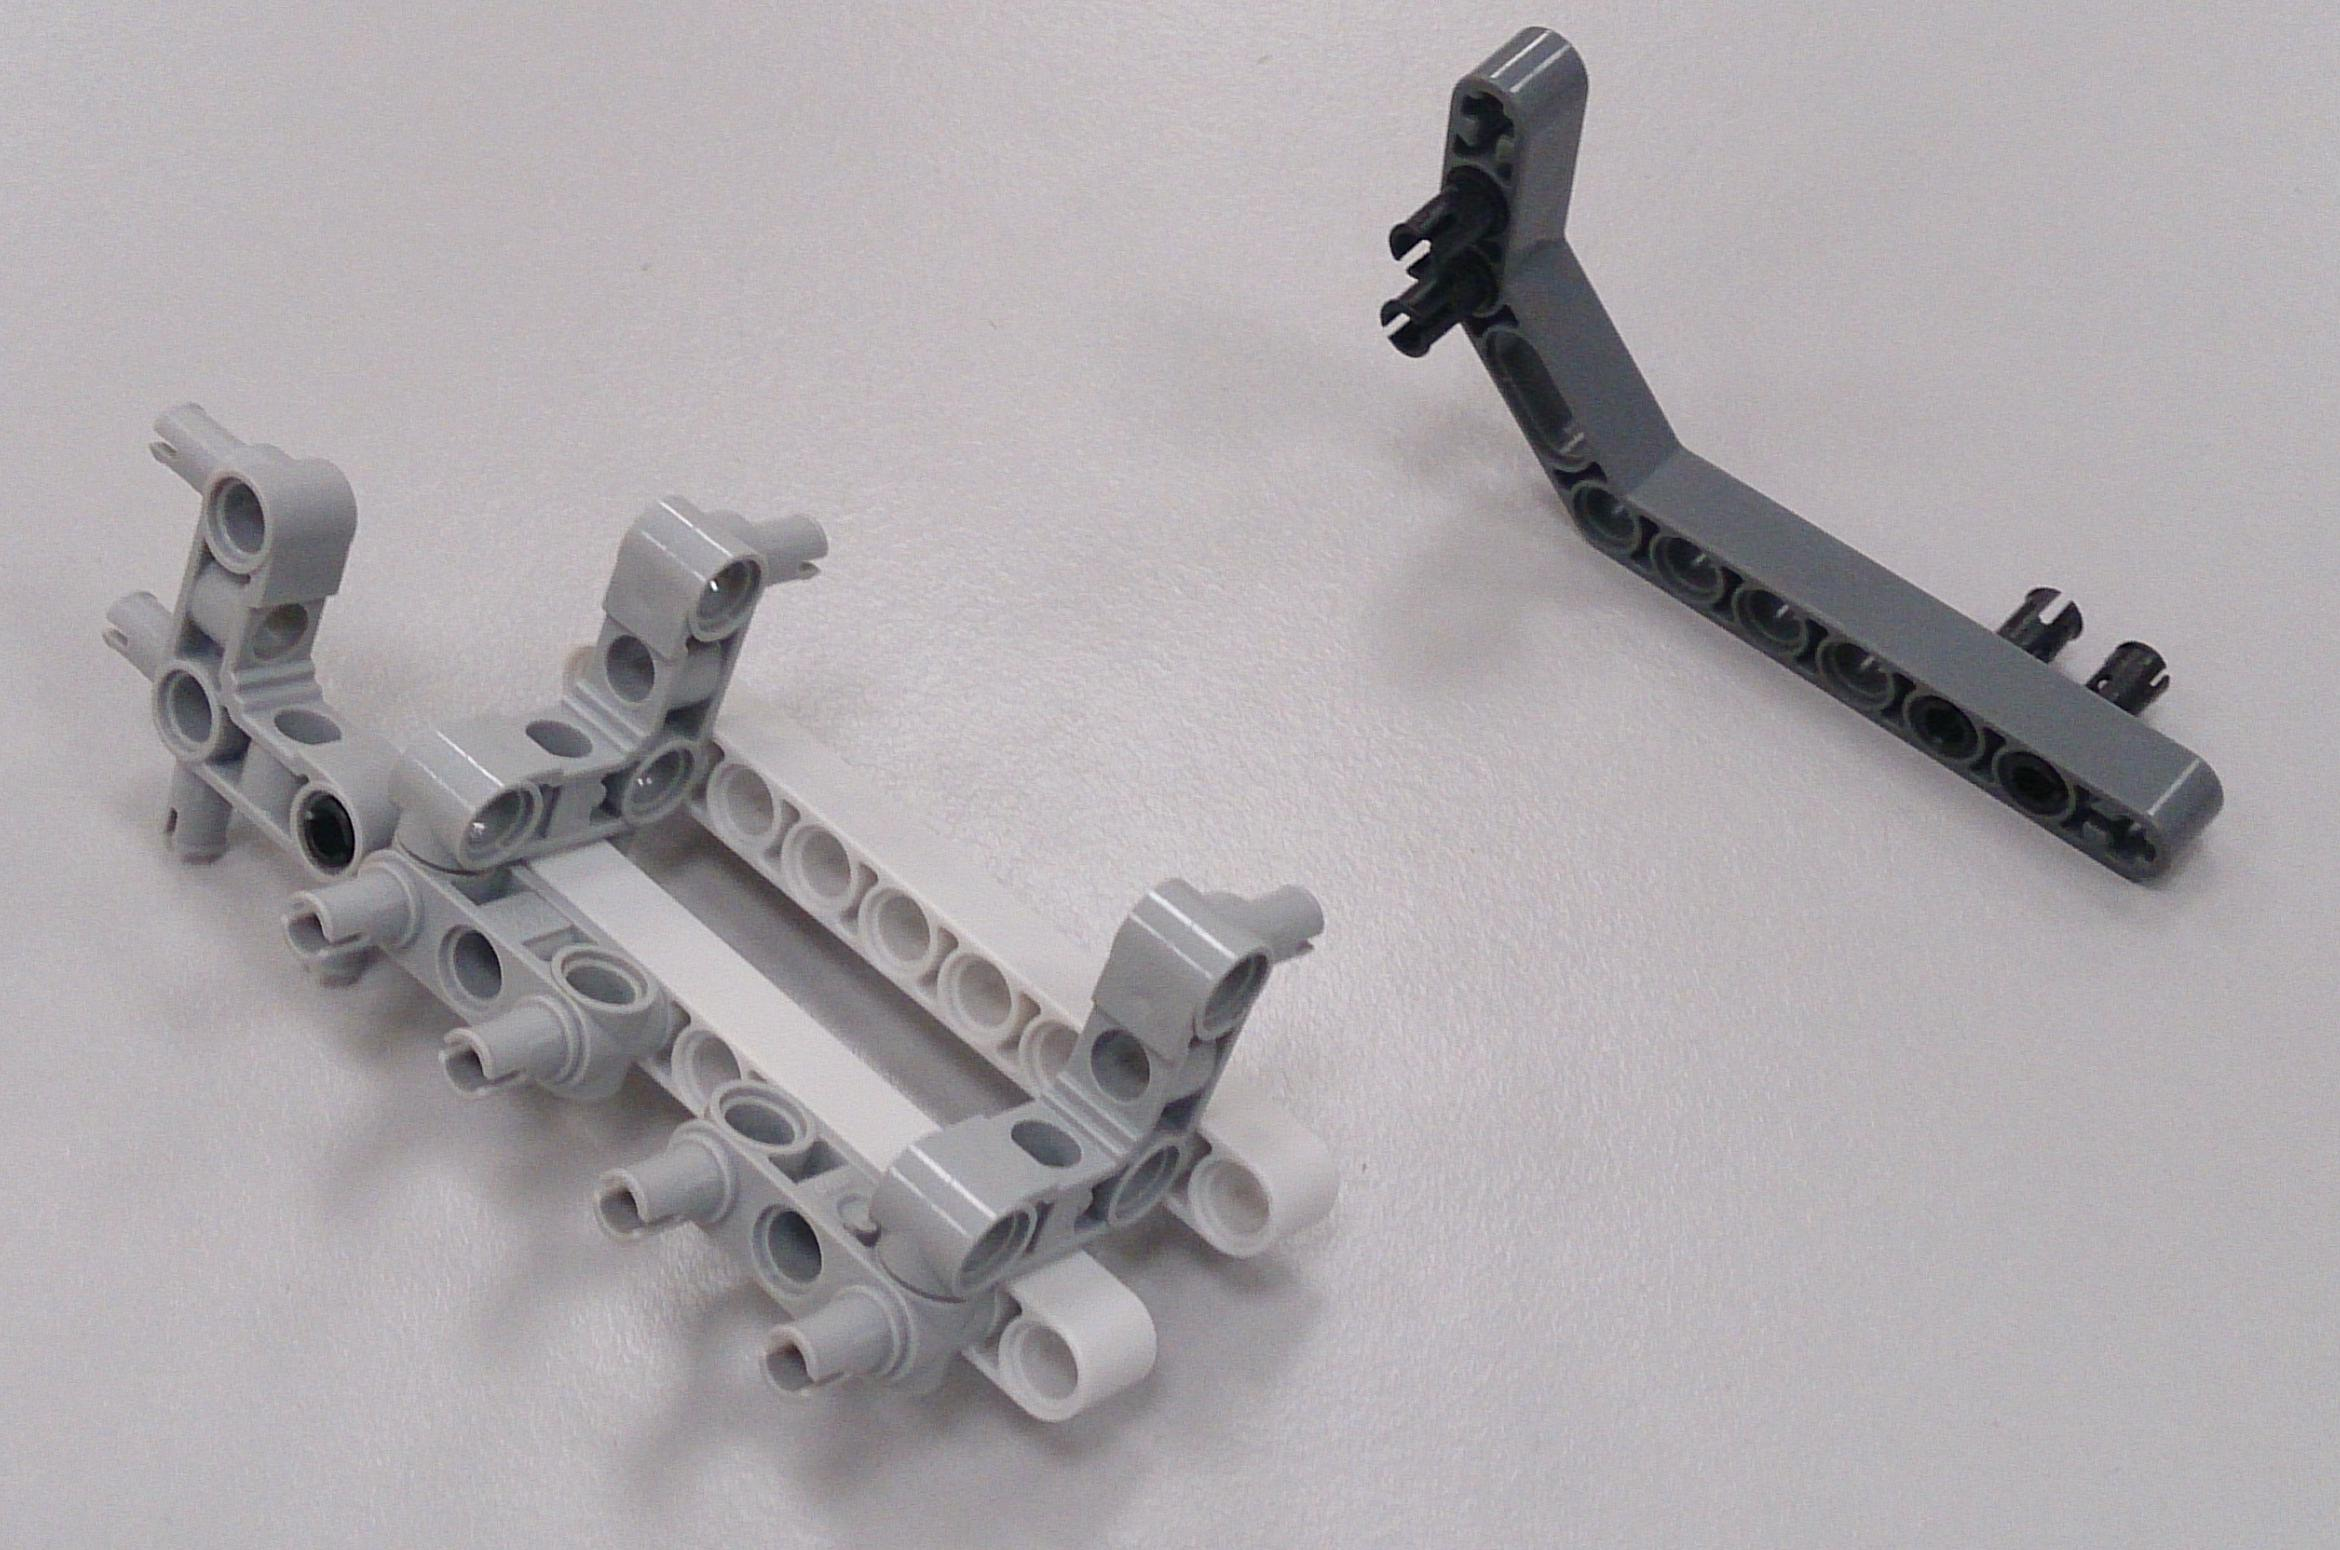
\includegraphics[height = 5.5 cm]{second.jpg} \\ б)}
	\end{minipage}
	\caption{Командный блок NXT и крепления для одного из двигателей.}
	\label{fig:first_pict_in_constr_example}
\end{figure}
\vfill
\begin{figure}[h]
	\begin{minipage}[h]{0.49\linewidth}
		\center{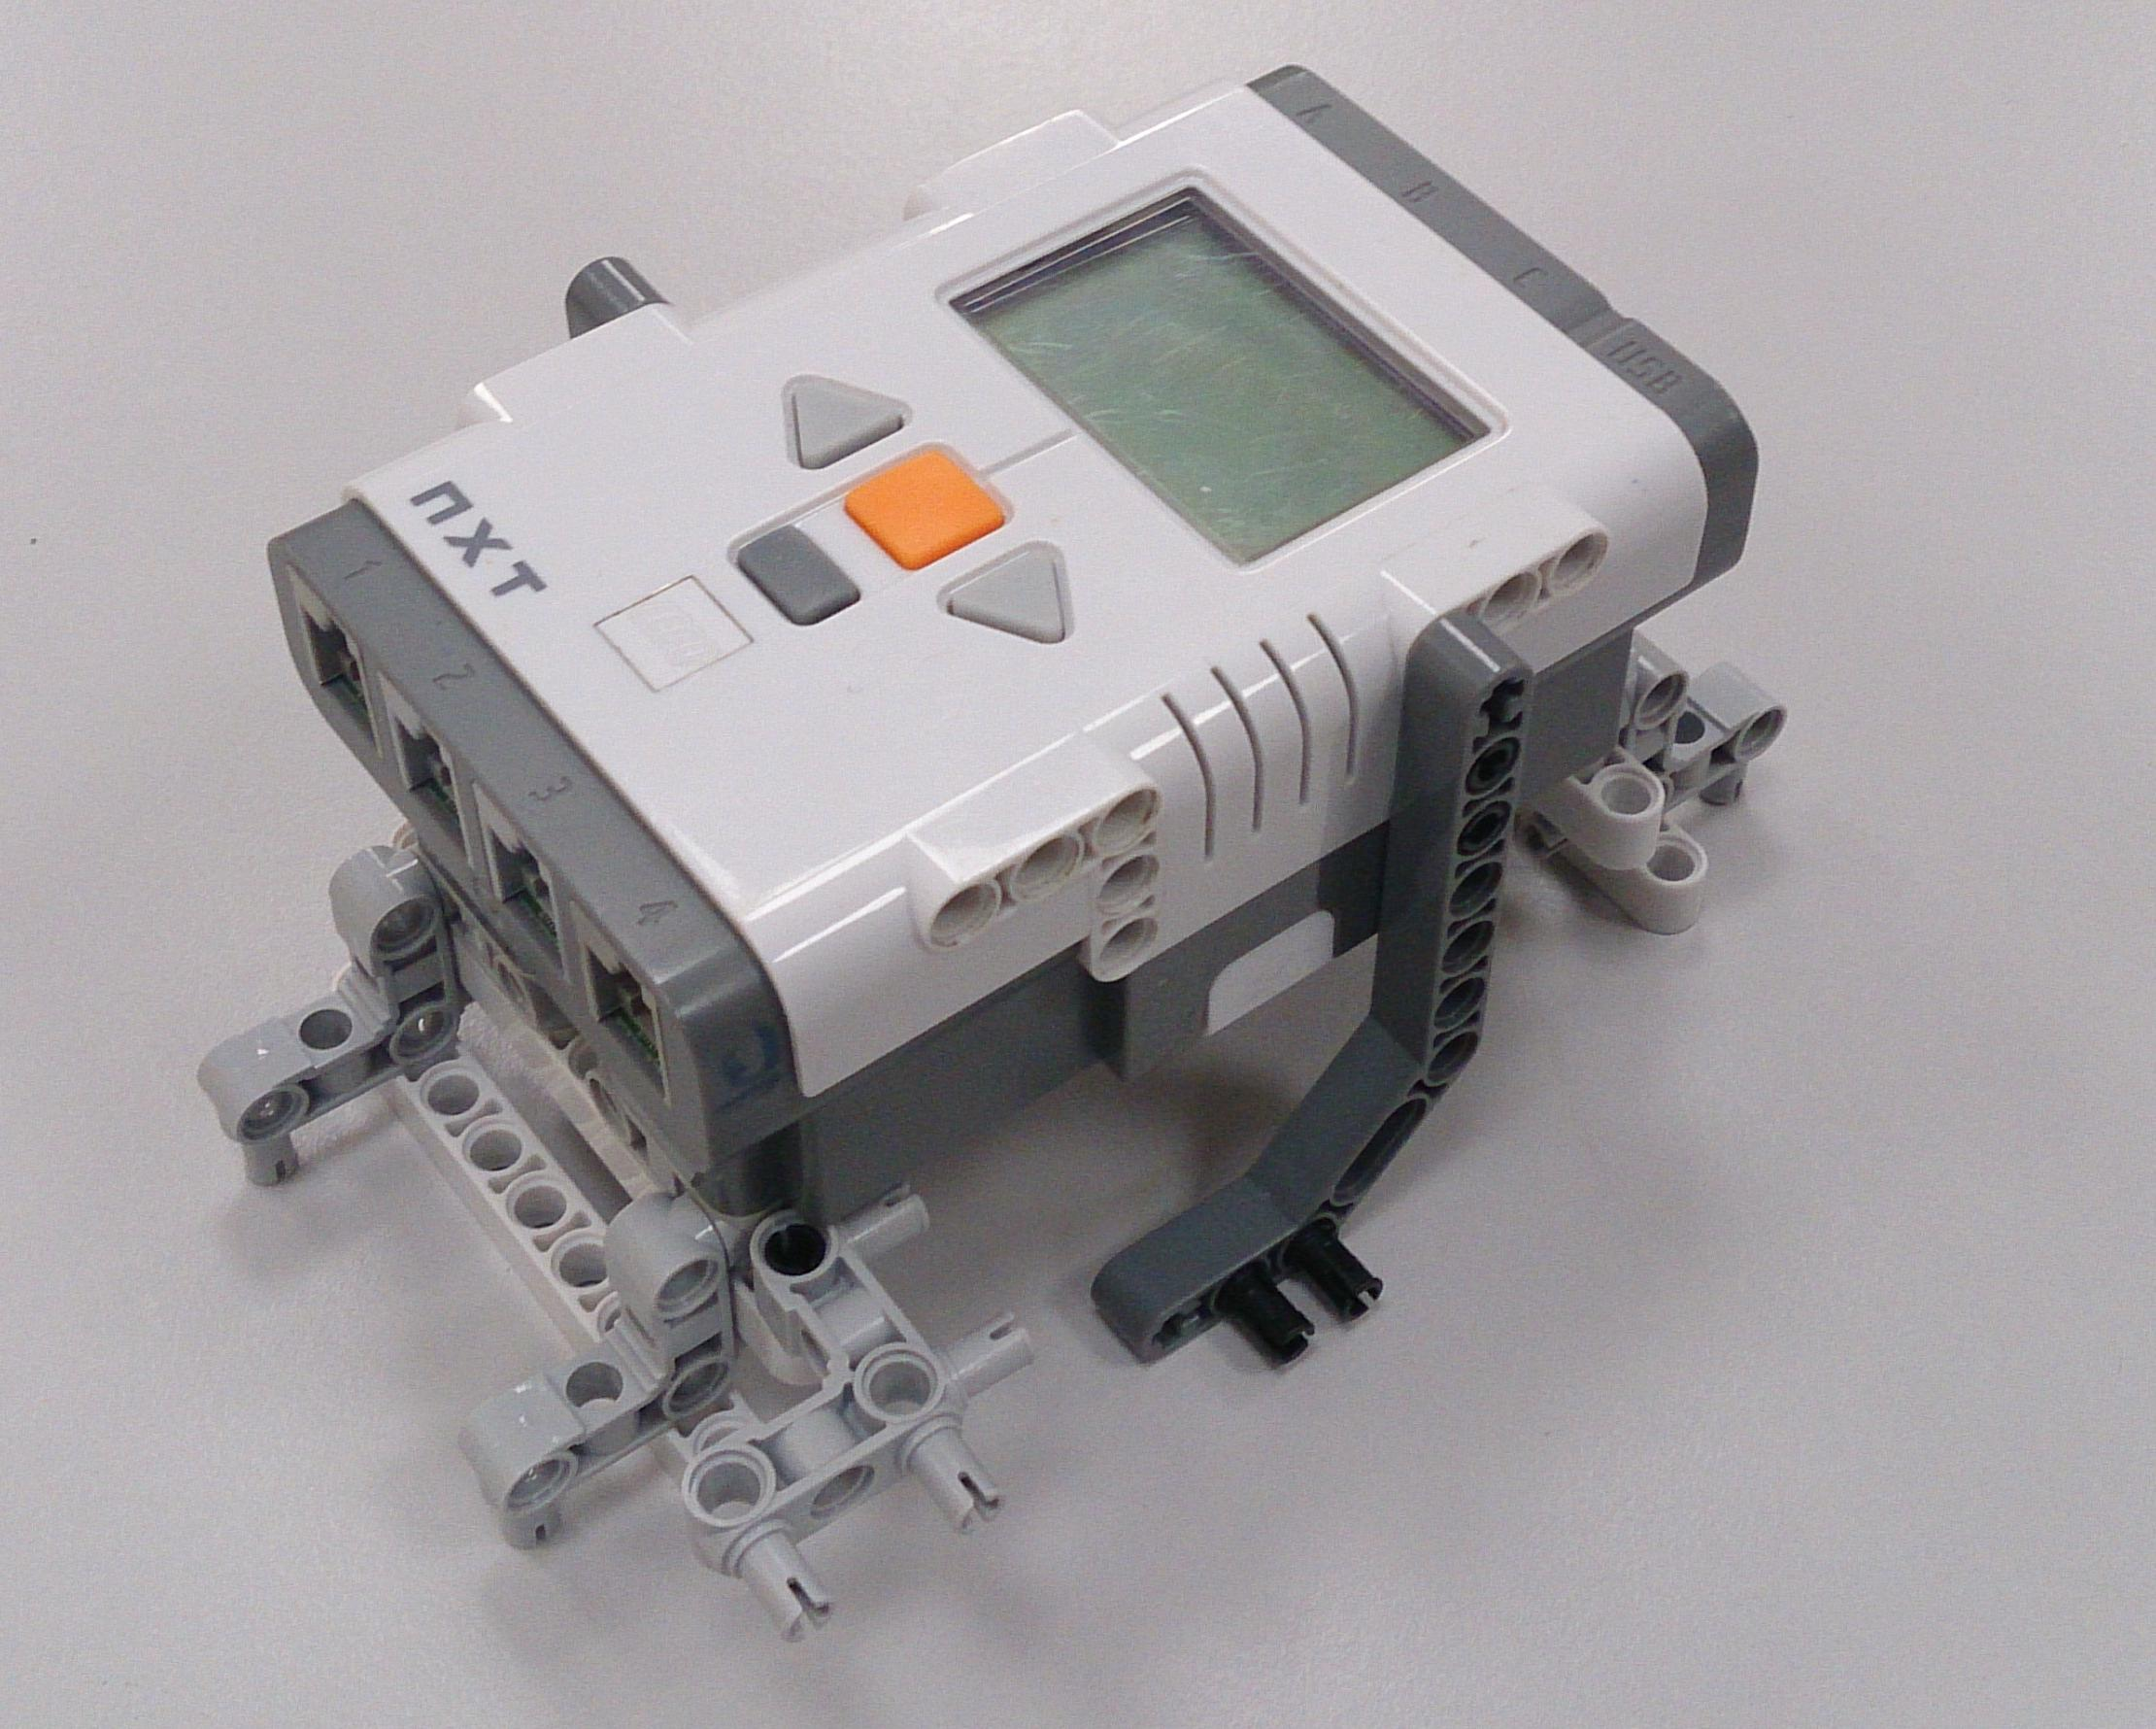
\includegraphics[height = 5.5 cm]{third.jpg} \\ а)}
	\end{minipage}
	\hfill
	\begin{minipage}[h]{0.49\linewidth}
		\center{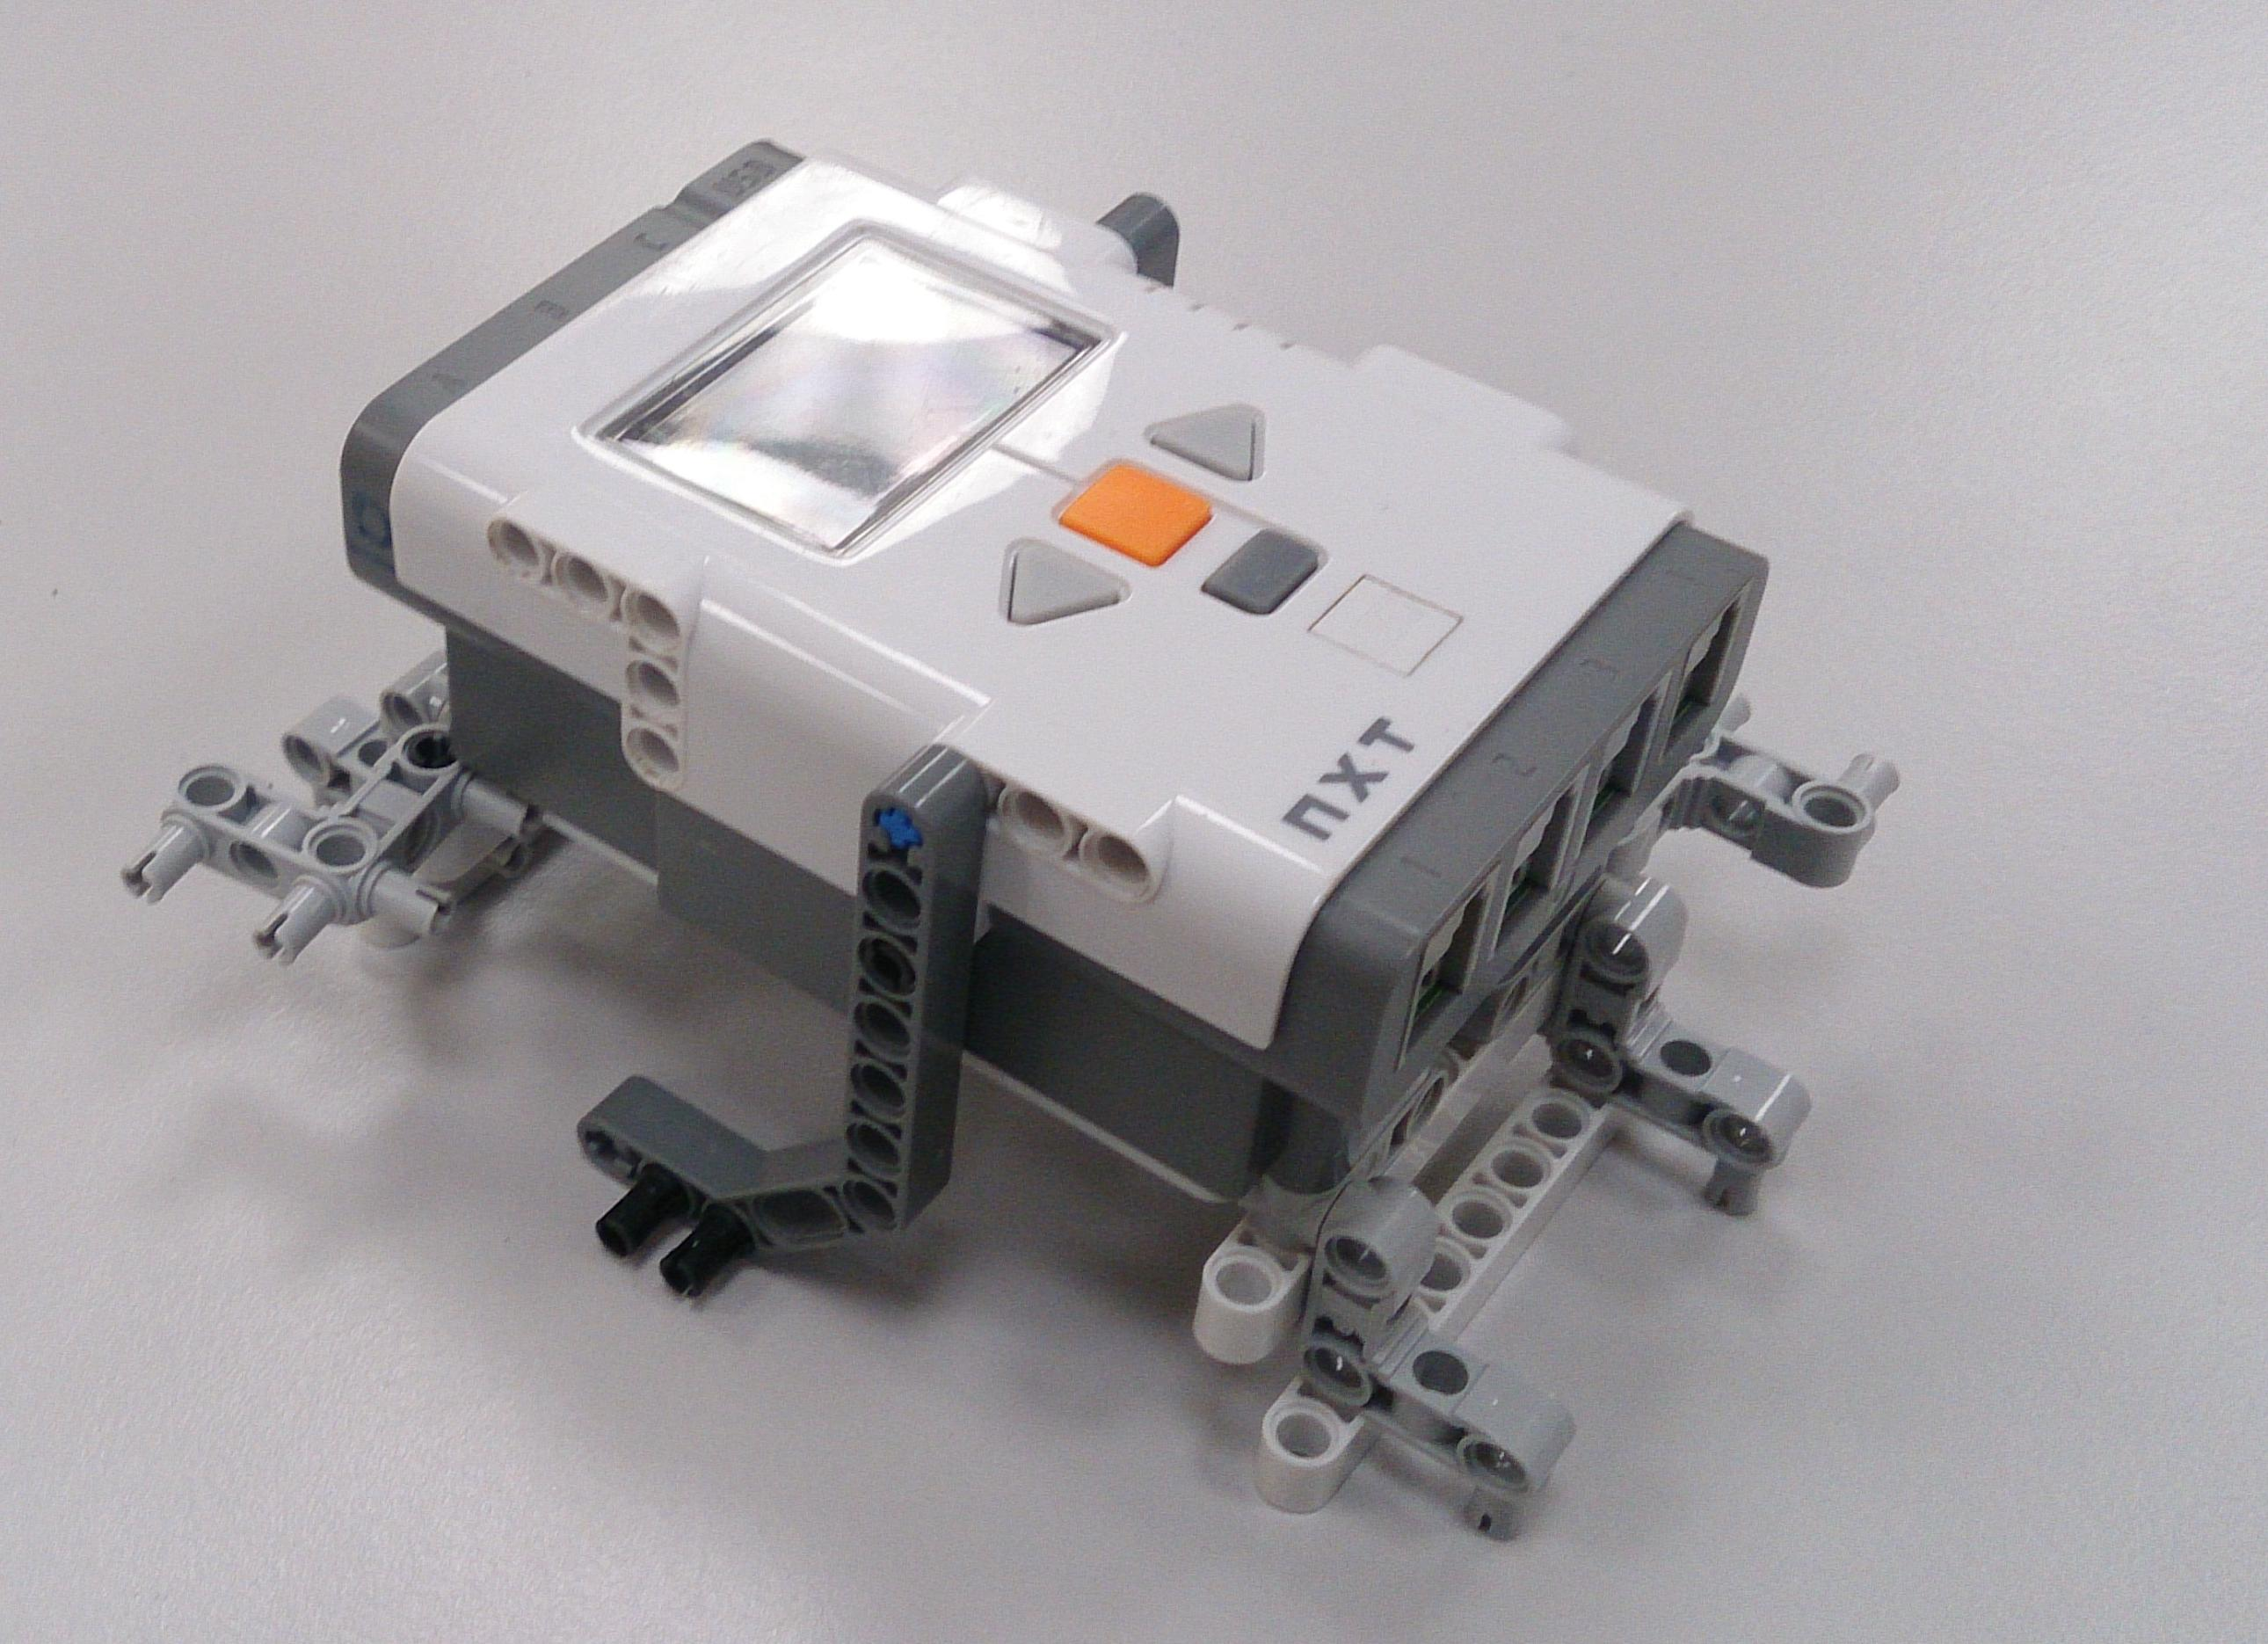
\includegraphics[height = 5.5 cm]{fourth.jpg} \\ б)}
	\end{minipage}
	\caption{Командный блок NXT с присоединенными к нему креплениями для двигателей.}
\end{figure}
\vfill

\begin{figure}[h]
	\noindent\centering{ 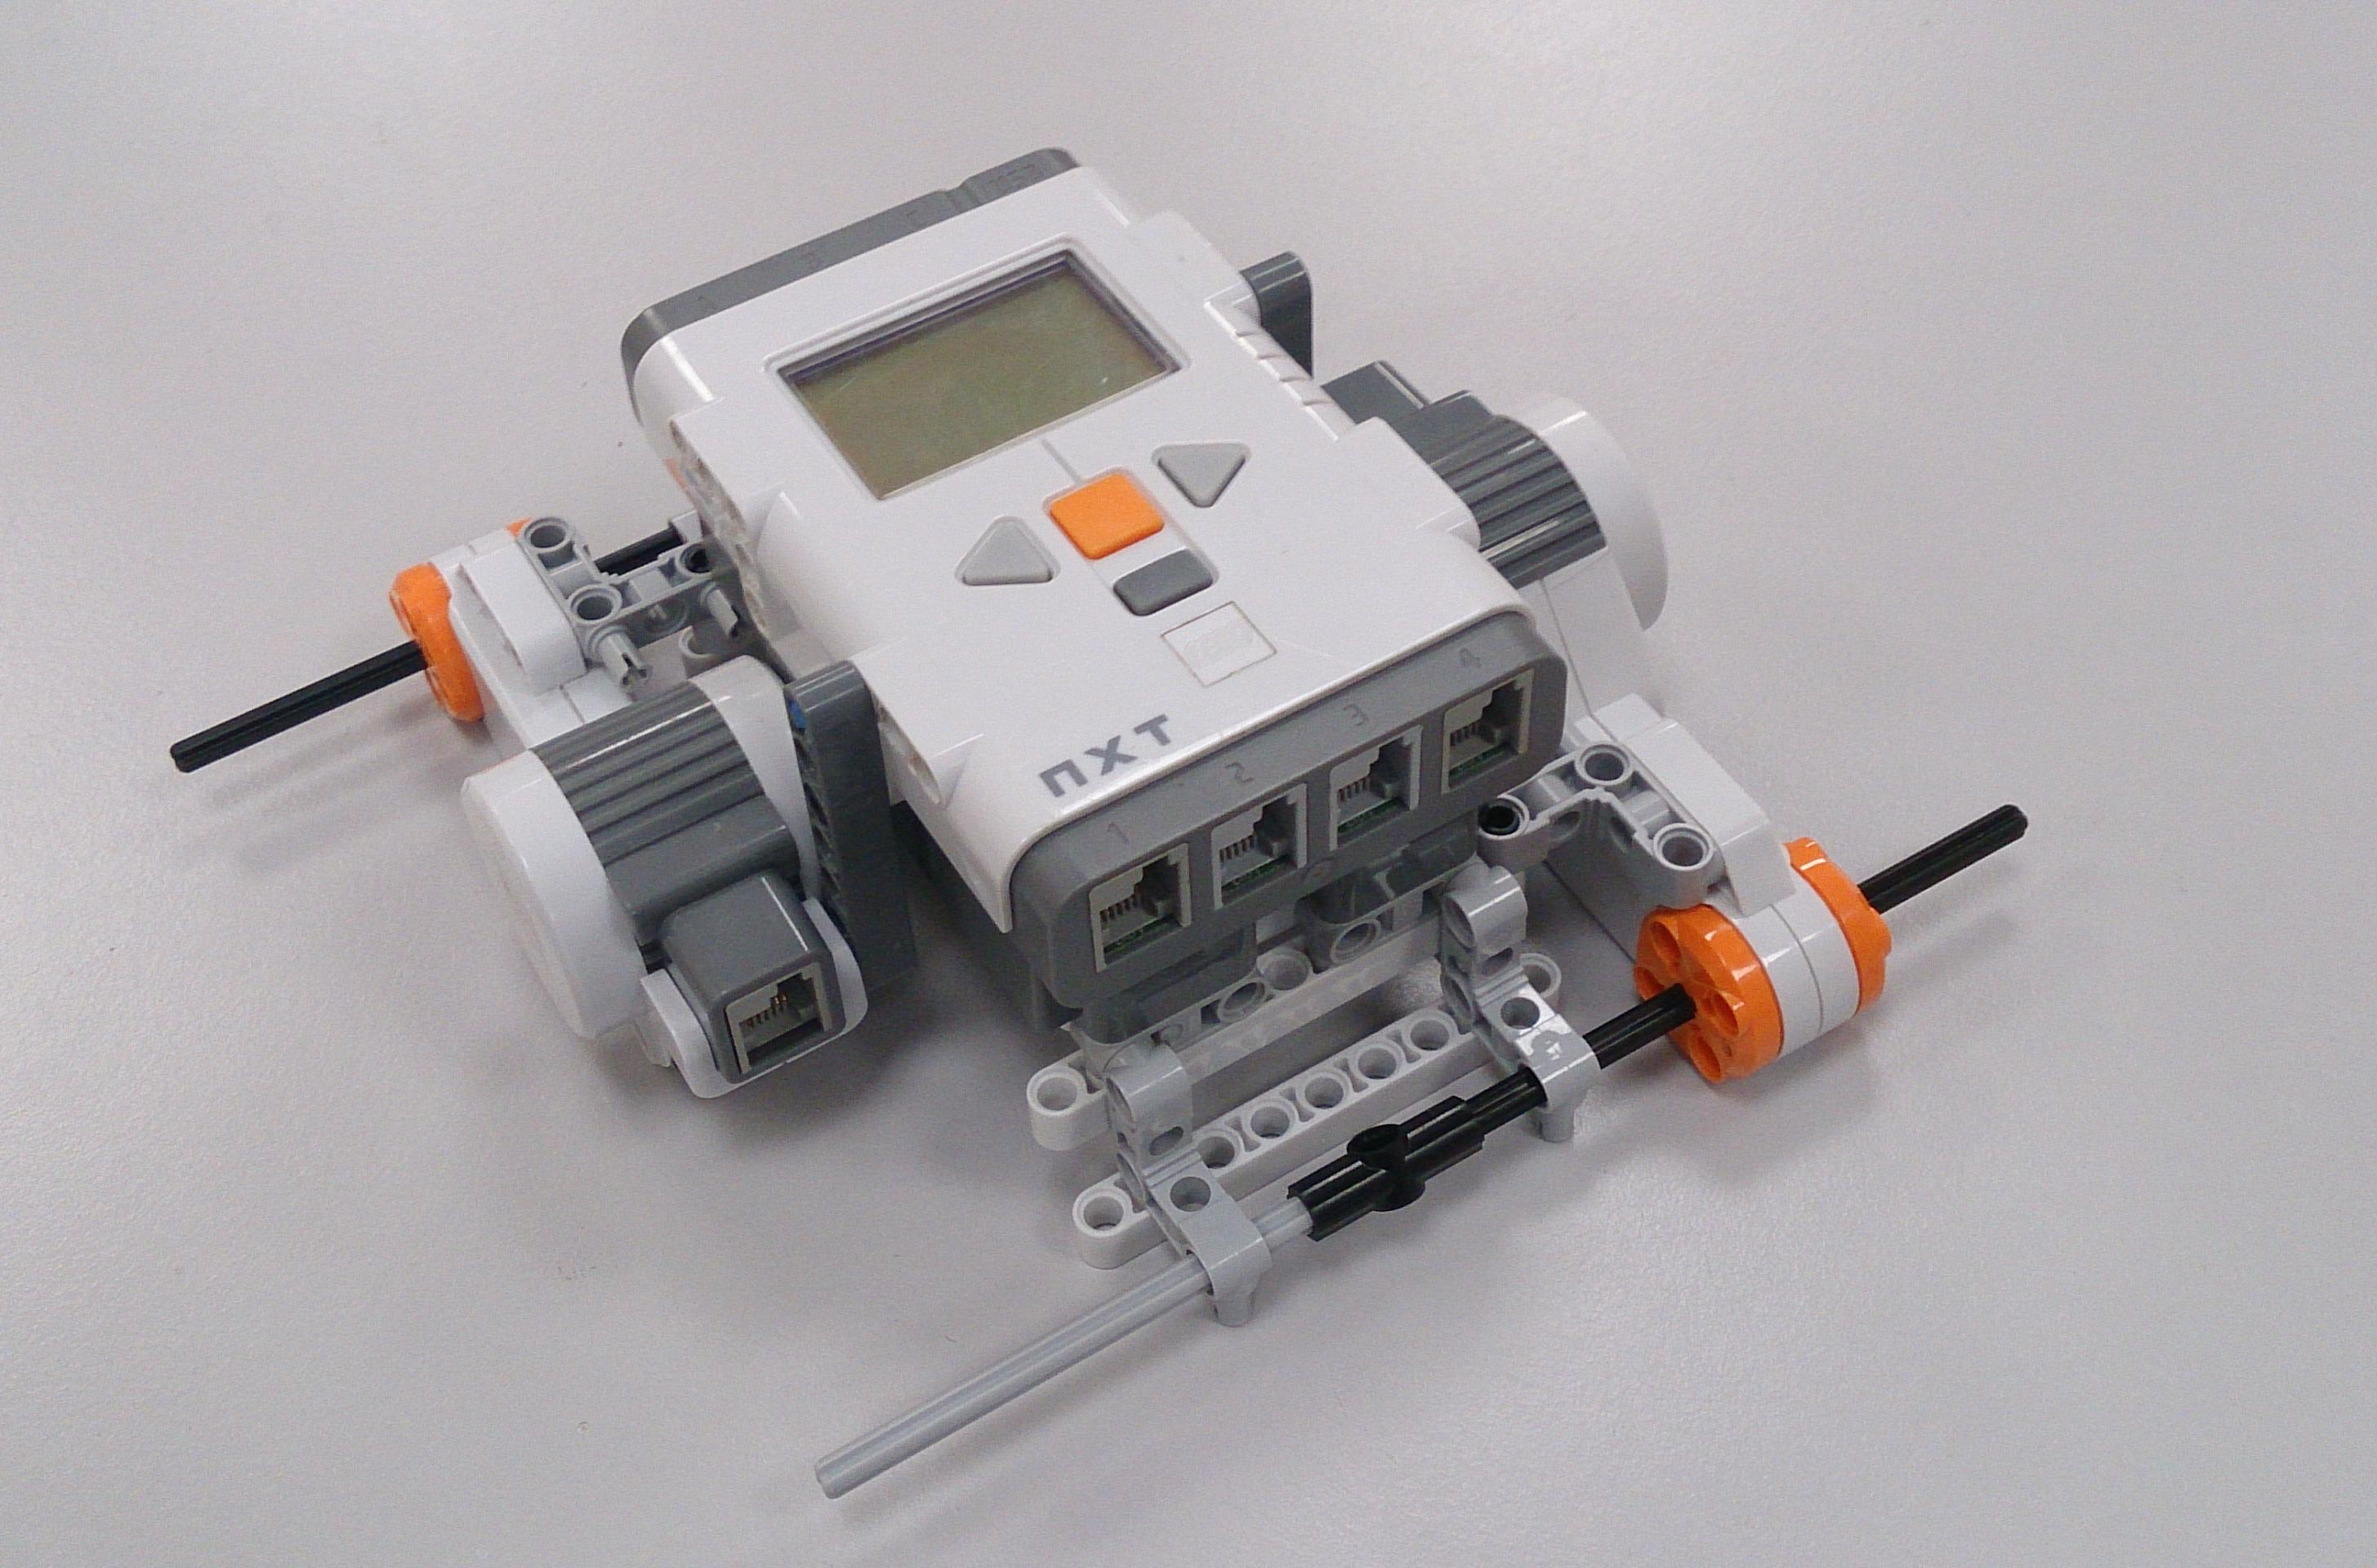
\includegraphics[width = \textwidth]{fifth.jpg} }
	\caption{Установка на робота двигателей.}
\end{figure}

\begin{figure}[h]
	\begin{minipage}[h]{0.49\linewidth}
		\flushleft {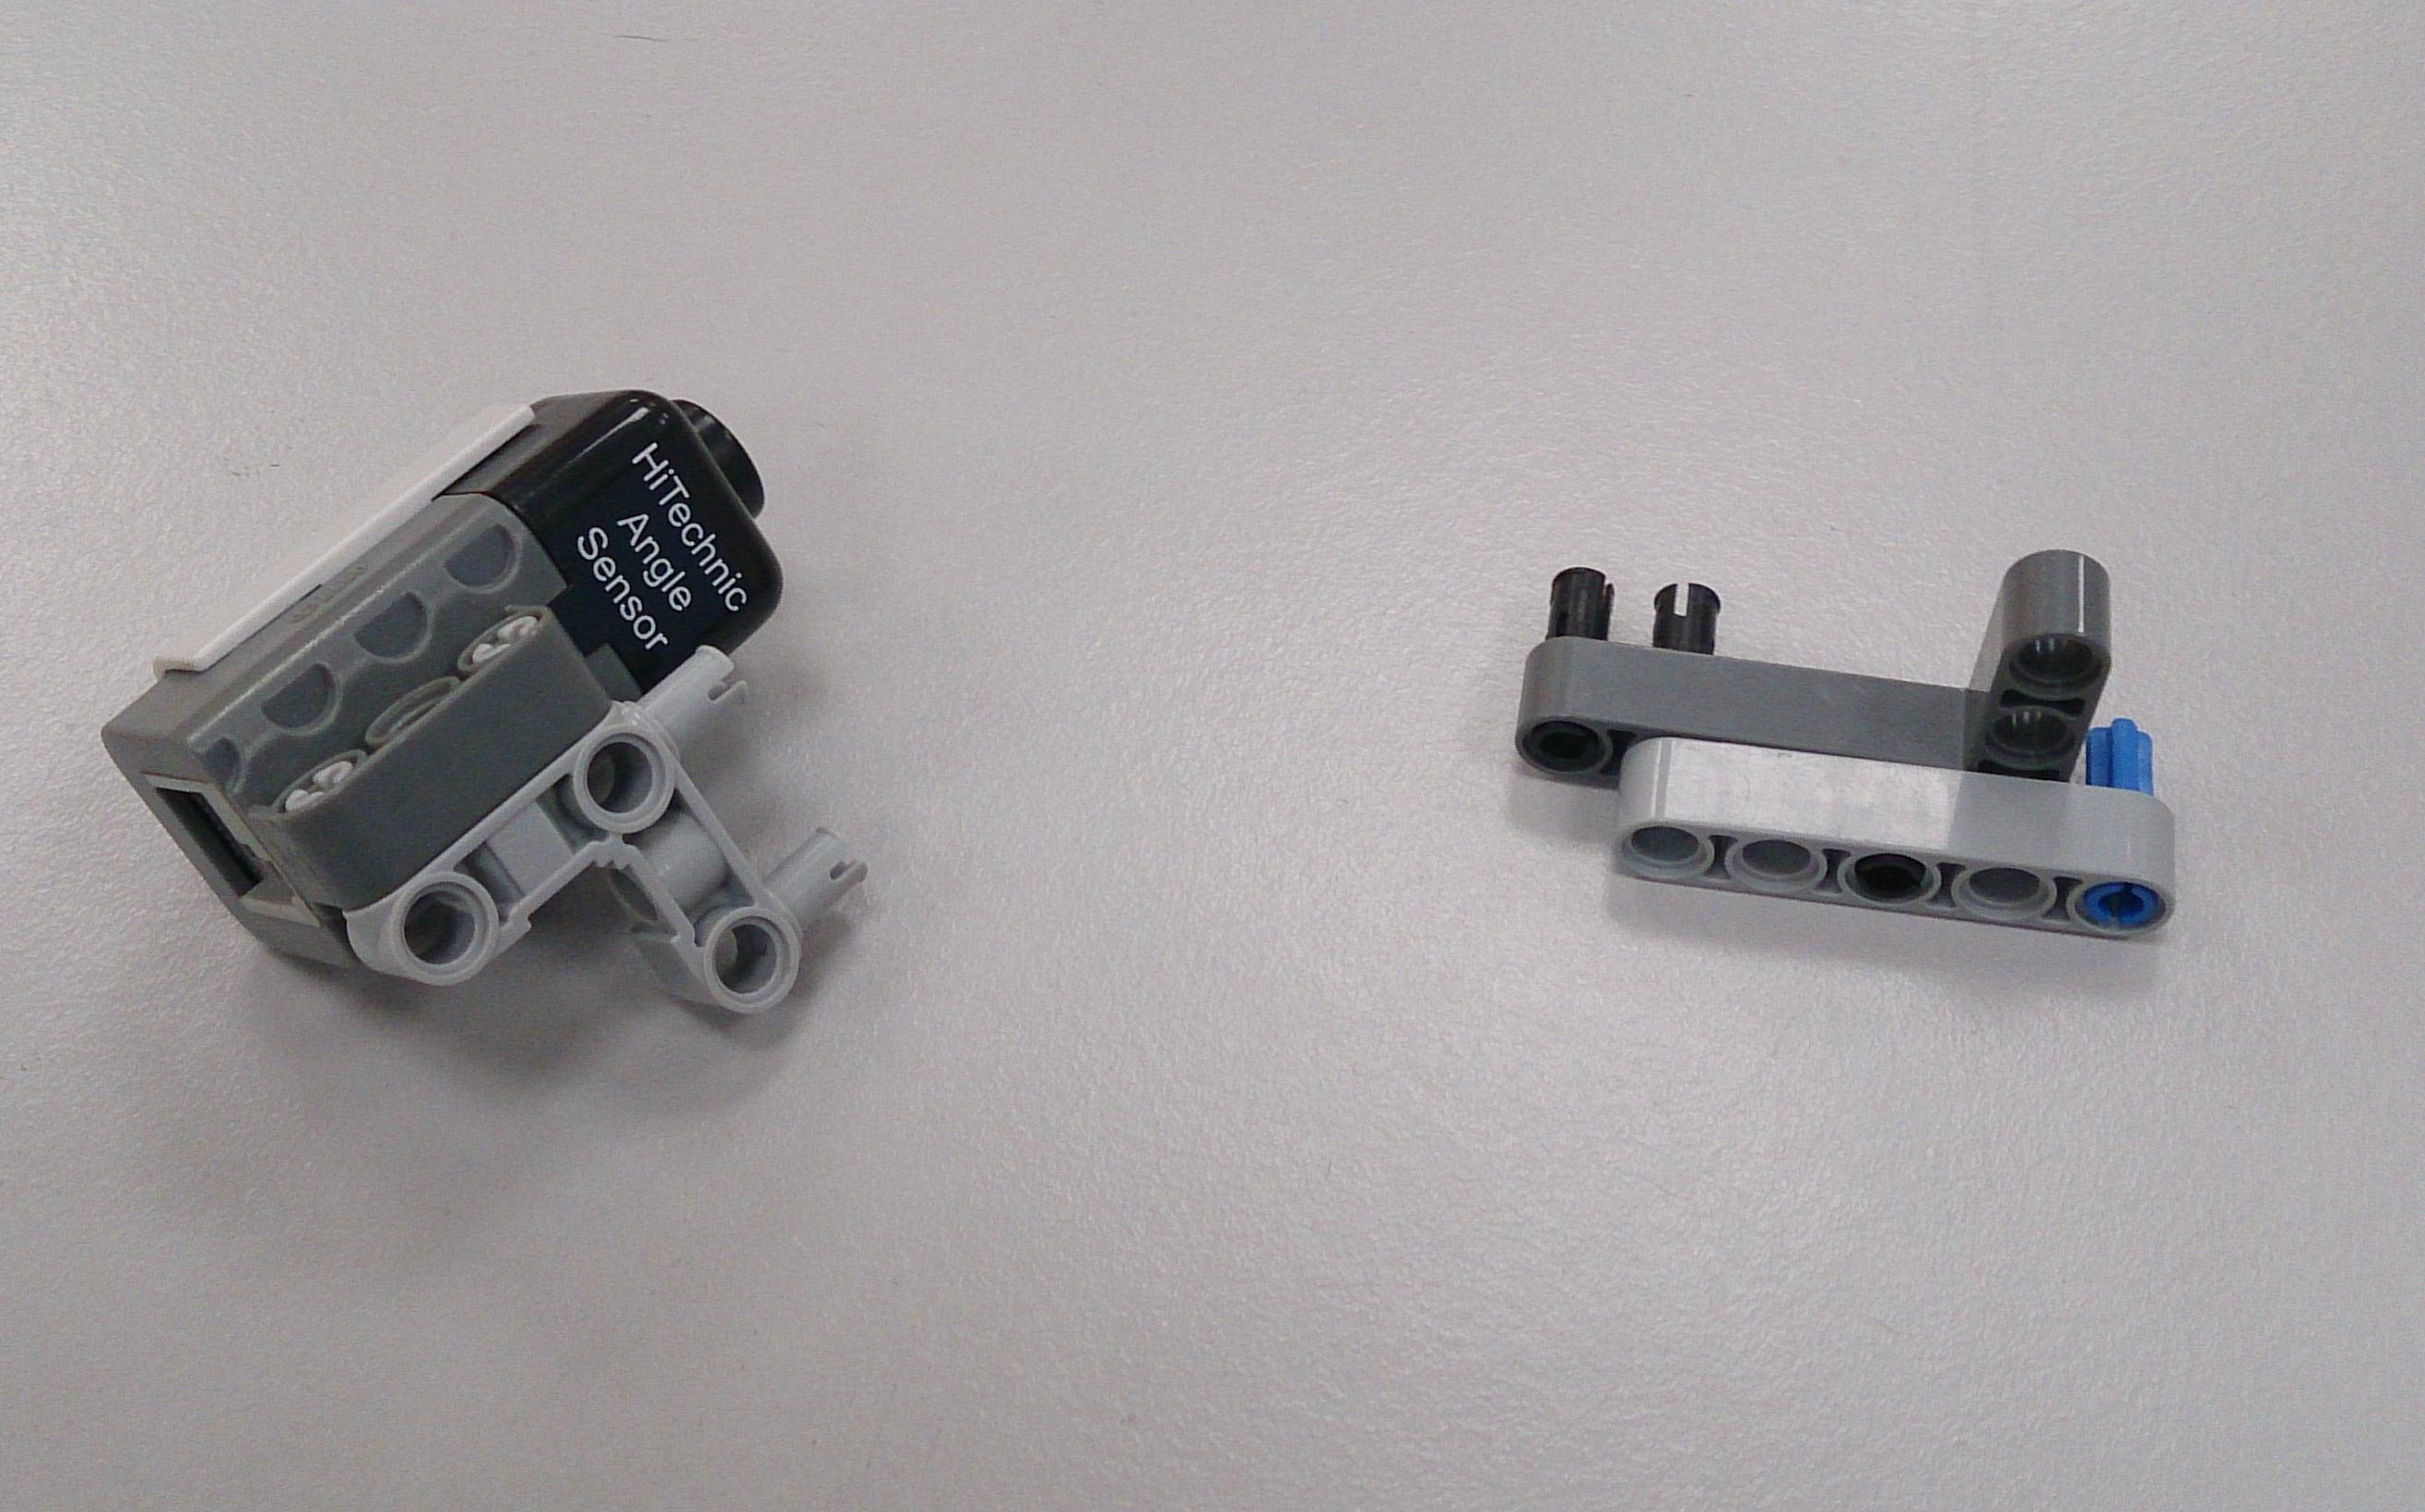
\includegraphics[height = 5.8 cm]{sixth.jpg} }\\ \centering{ а)}
	\end{minipage}
	\hfill
	\begin{minipage}[h]{0.49\linewidth}
		\flushright {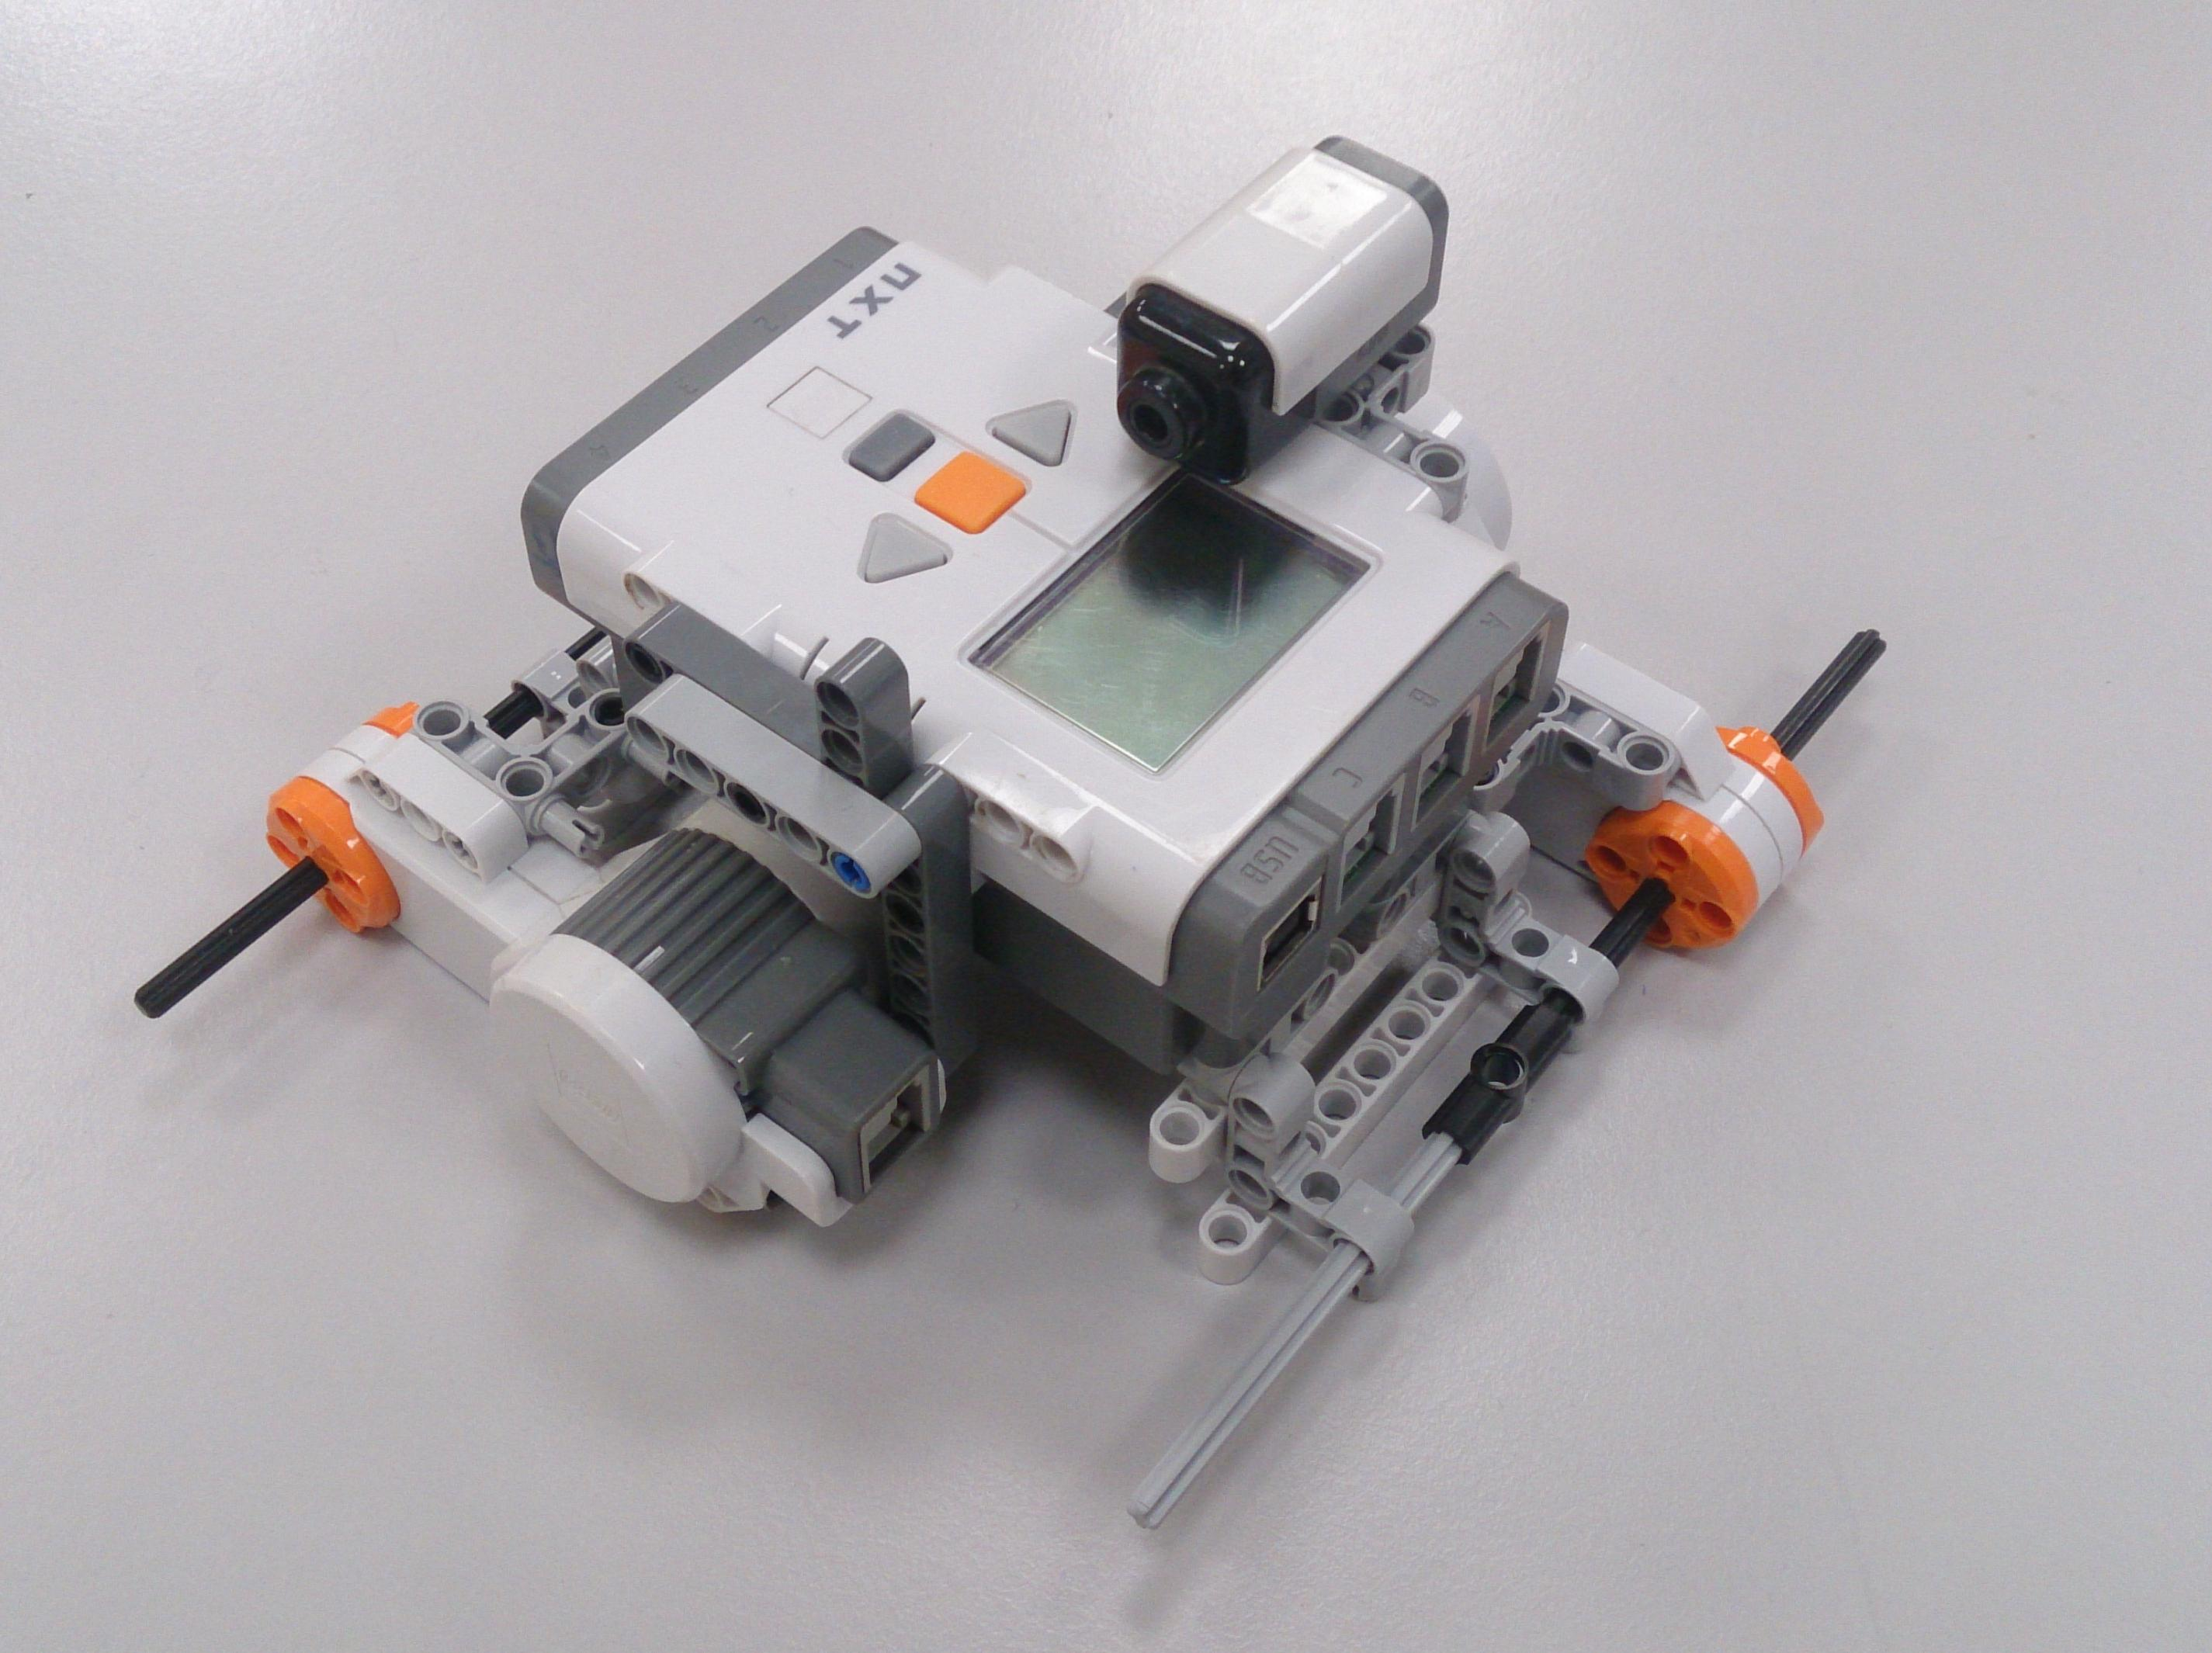
\includegraphics[height = 5.8 cm]{seventh.jpg} } \\ \centering{ б)}
	\end{minipage}
	\caption{Установка креплений для оси вращения маятника.}
\end{figure}

\begin{figure}[h]
	\noindent\centering{ 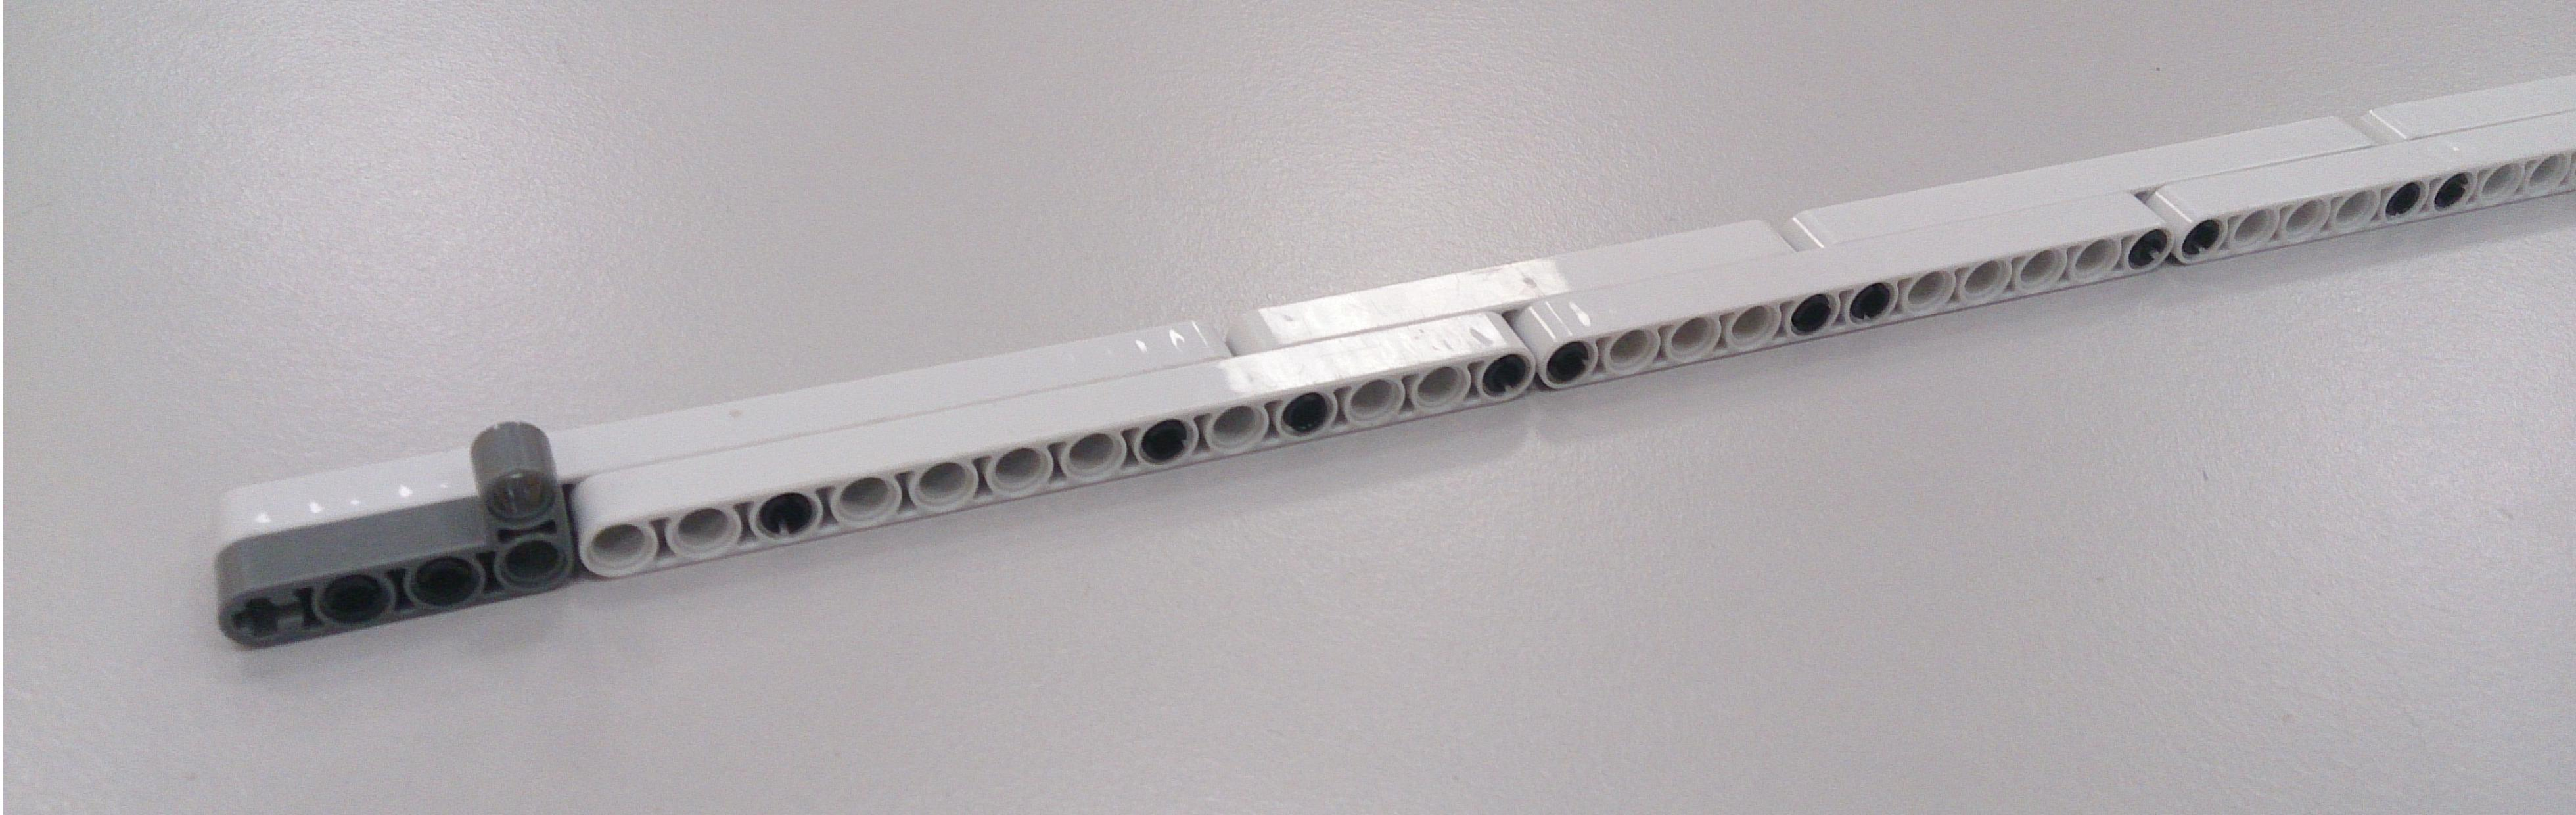
\includegraphics[width = \textwidth]{eighth.jpg} }
	\caption{Конец маятника с крепежным пазом.}
\end{figure}

\begin{figure}[h]
	\noindent\centering{ 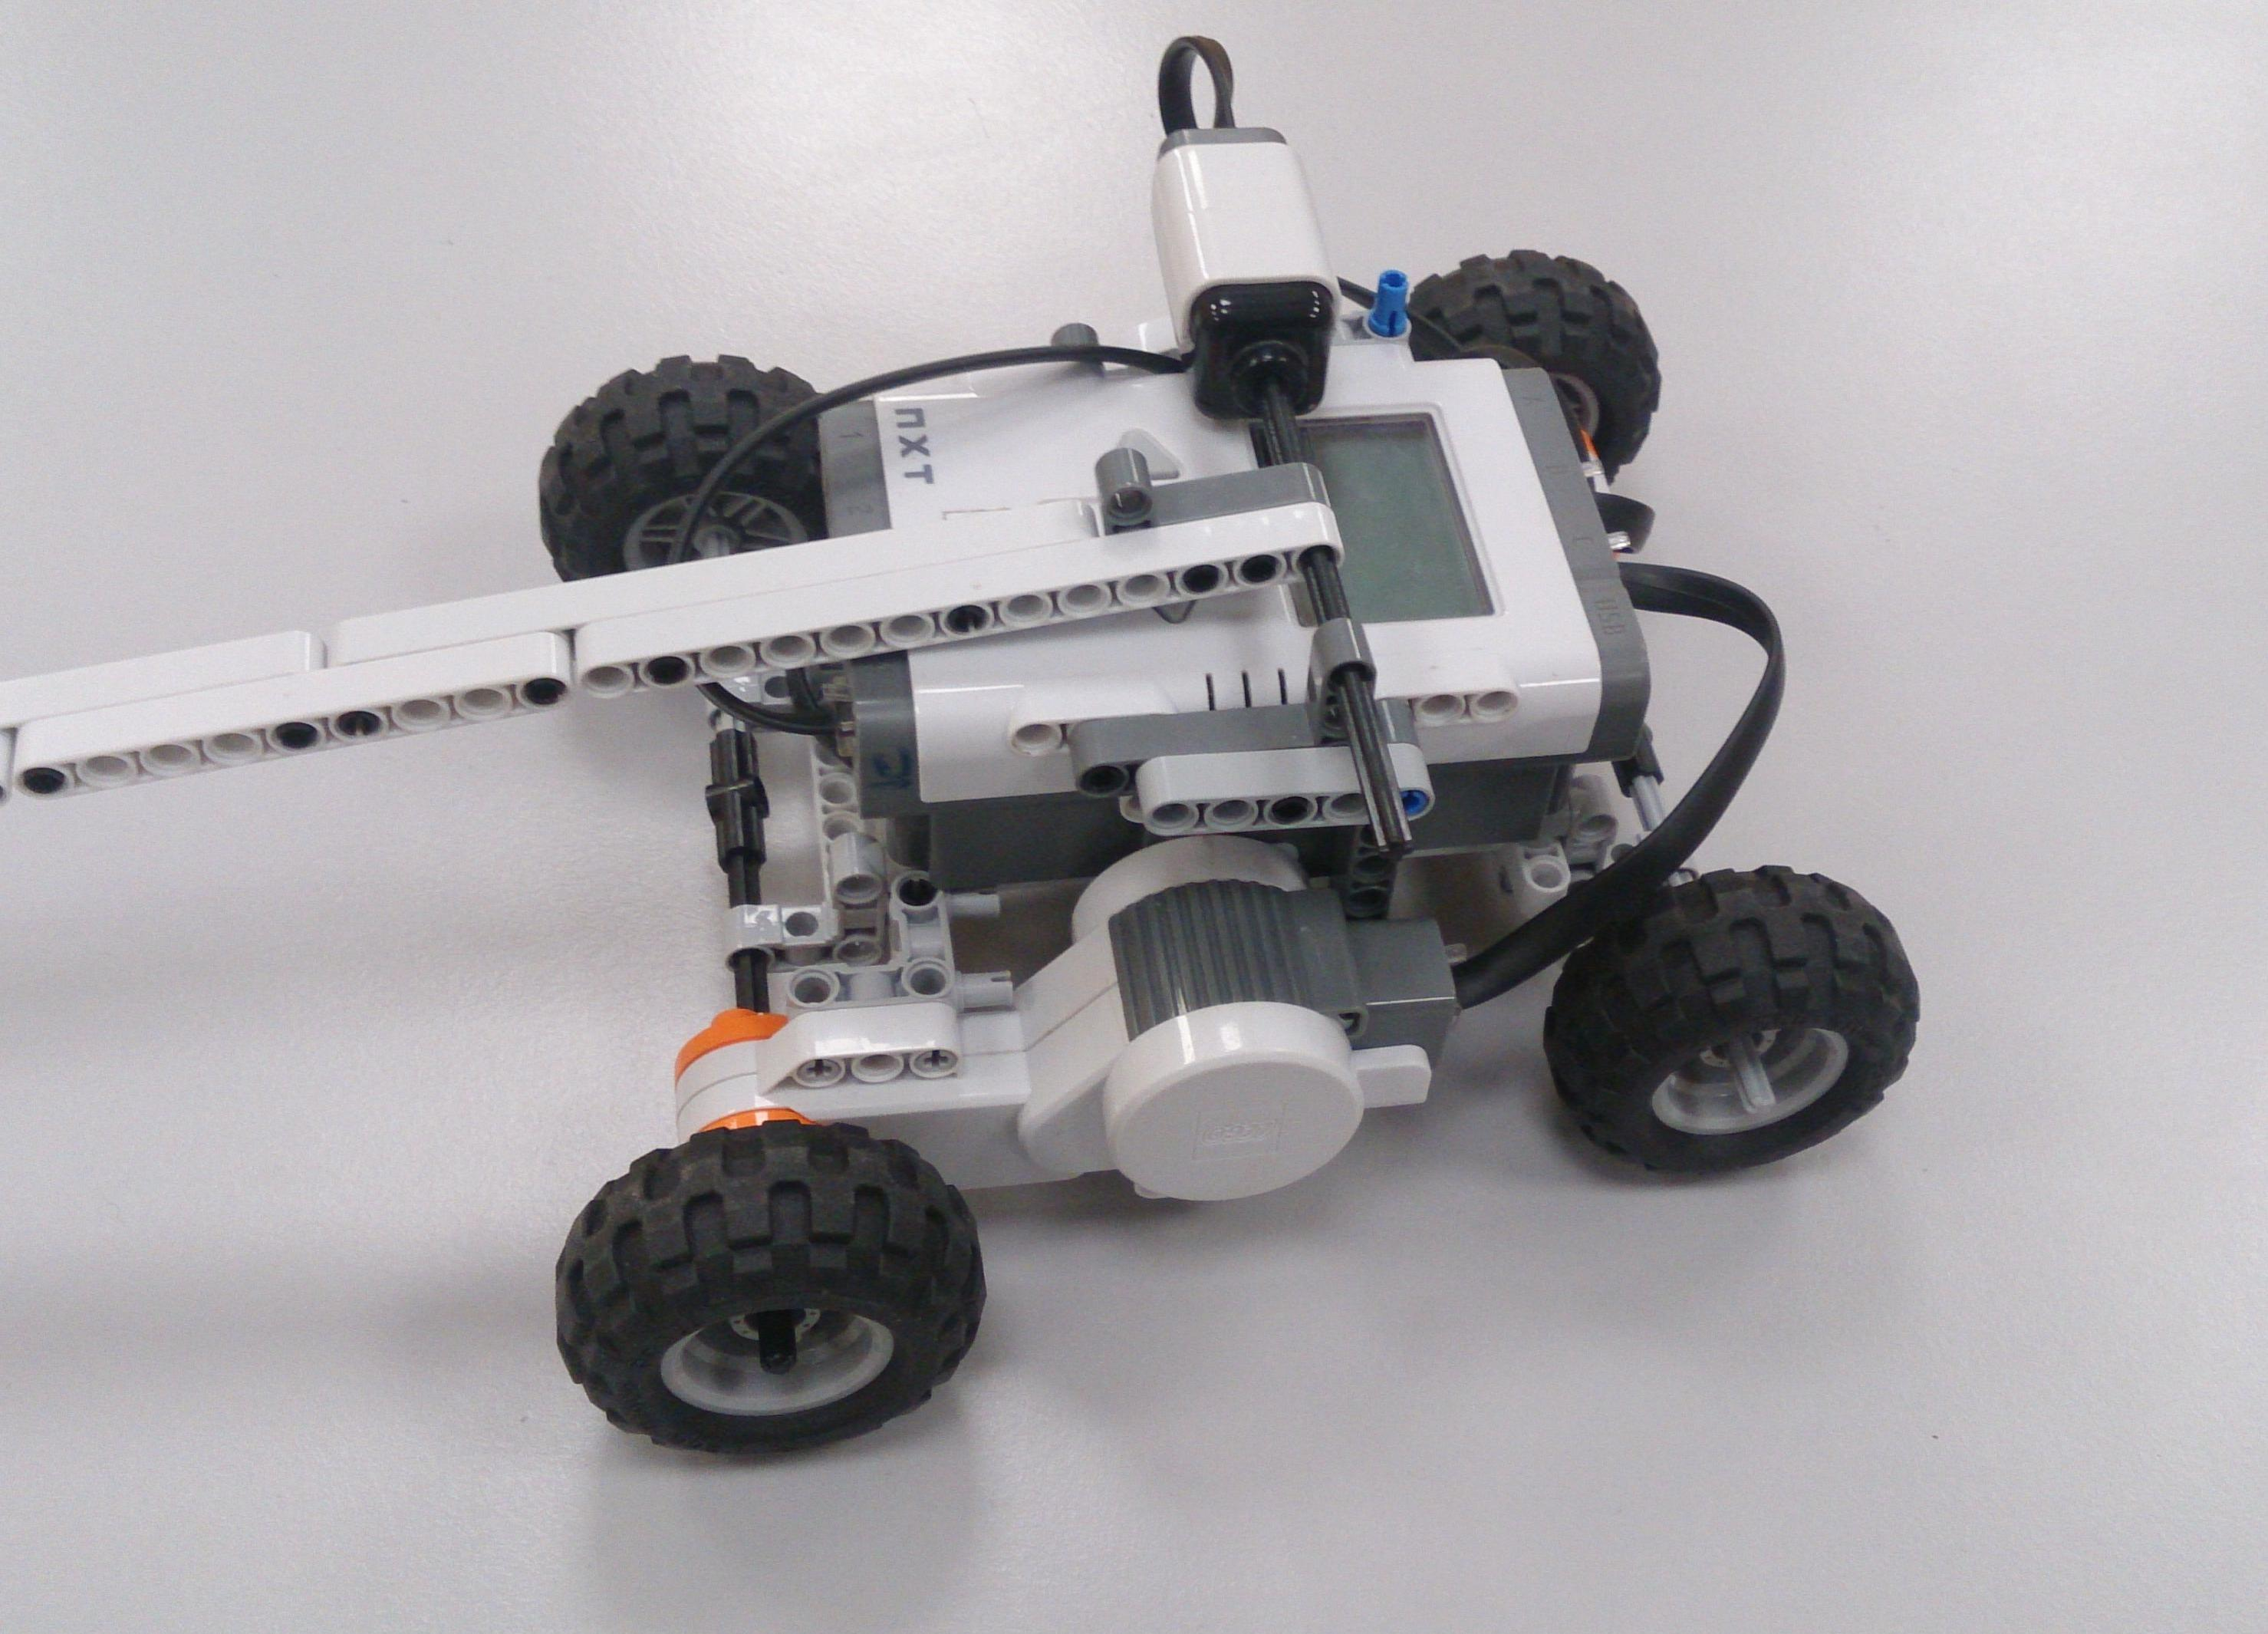
\includegraphics[width = \textwidth]{ninth.jpg} }
	\caption{Полностью собранный робот.}
	\label{fig:last_pict_in_constr_example}
\end{figure}

\end{document}

